\documentclass[a4paper,12pt]{article}
\usepackage[utf8]{inputenc}
\usepackage[german]{babel}
\usepackage{amsmath}
\usepackage{amssymb}
\usepackage{amsthm}
\usepackage{geometry}
\usepackage{graphicx}
\usepackage[hidelinks]{hyperref}
\usepackage{listings}
\usepackage{xcolor}
\usepackage{microtype}
\usepackage{enumitem}
\usepackage{tikz}
\usepackage{booktabs}
\usetikzlibrary{arrows.meta, positioning, shapes.geometric, fit, calc}

\geometry{margin=2.5cm}

\theoremstyle{definition}
\newtheorem{definition}{Definition}
\newtheorem{beispiel}{Beispiel}
\newtheorem{satz}{Satz}
\newtheorem{lemma}{Lemma}
\newtheorem{korollar}{Korollar}
\newtheorem{bemerkung}{Bemerkung}
\newtheorem{theorem}{Theorem}

\setlist[itemize,1]{label=--}

\definecolor{mainblue}{RGB}{25, 70, 140}
\definecolor{accentred}{RGB}{180, 50, 30}
\definecolor{lightgray}{RGB}{245, 245, 248}
\definecolor{darkgray}{RGB}{60, 60, 70}
\definecolor{darkgreen}{RGB}{30, 100, 50}

\hypersetup{
    colorlinks=true,
    linkcolor=mainblue,
    citecolor=accentred,
    urlcolor=mainblue,
    pdftitle={Reduktionen beim Java-Compilerbau auf das Subgraph-Isomorphismusproblem},
    pdfauthor={Stephan Epp},
}

\lstset{
    columns=flexible,
    basicstyle=\ttfamily\small,
    keywordstyle=\color{blue},
    commentstyle=\color{gray},
    stringstyle=\color{accentred},
    numbers=left,
    numberstyle=\tiny,
    breaklines=true,
    frame=single,
    literate=%
    {Ö}{{\"O}}1 {Ä}{{\"A}}1 {Ü}{{\"U}}1
    {ß}{{\ss}}1 {ü}{{\"u}}1 {ä}{{\"a}}1 {ö}{{\"o}}1
}

\lstdefinestyle{javastyle}{
    language=Java,
    morekeywords={var, record, sealed, permits, yield},
    keywordstyle=\color{mainblue}\bfseries,
}

\lstdefinestyle{bashstyle}{
    language=bash,
    morekeywords={javac, java, mvn, gradle},
    keywordstyle=\color{darkgreen}\bfseries,
}

\title{\textbf{Reduktionen beim Java-Compilerbau\\
auf das Subgraph-Isomorphismusproblem}\\[0.1em]
\large Formale Beweise, Java-Implementierung und Ausblick}
\author{Stephan Epp}
\date{23. Juni 2026}

\begin{document}
\sloppy
\maketitle
\tableofcontents
\newpage

%=====================================================================
\section{Einf\"uhrung}
%=====================================================================

Diese Arbeit entwickelt eine vollst\"andige, formal bewiesene
Reduktionstheorie zwischen zentralen komplexit\"atstheoretischen
Problemen beim Java-Compilerentwurf einerseits und dem
Subgraph-Iso\-morphismusproblem andererseits.  Wir zeigen, dass acht
fundamentale Probleme -- Typaufl\"osung und Vererbungshierarchie (TAP),
Dead-Code-Elimination (DCE), Konstantenpropagation in SSA-Form (CPP),
Registerallokation f\"ur die JVM (RAP), Schleifenoptimierung mittels
Dominatorgraph (SEP), Modulabh\"angigkeitsaufl\"osung im Java Platform
Module System (LAP), statische Initialisierungsreihenfolge (IRP) und
Bytecode-Verifikation (BVP) -- jeweils in polynomieller Zeit auf das
Subgraph-Isomorphismusproblem reduzierbar sind.  F\"ur jede Reduktion
liefern wir einen vollst\"andigen Korrektheitsbeweis, eine effiziente
L\"osung mittels des Subgraph Algorithmus (Epp~2026) \cite{epp2026}
sowie eine vollst\"andige Java-Implementierung des Demonstrations\-compilers
\textsc{jcl} (Java Compiler via Language-Graph).

Der Java-Compiler (\texttt{javac}) ist das produktionsreife
Referenzwerkzeug f\"ur die JVM-Plattform.  Dennoch bleiben die
graphentheoretischen Strukturen, die seinen internen Phasen zugrunde
liegen -- Vererbungsgraphen, Kontrollflussgraphen,
SSA-Abh\"angigkeitsgraphen, Interferenzgraphen -- oft ungenutzte
Quellen f\"ur einheitliche algorithmische Behandlung.  Der Subgraph
Algorithmus (Epp~2026) bietet eine einheitliche, effiziente Methode
zur L\"osung graphenstruktureller Fragen mit einer Laufzeit von
$O(n^3)$, die unter der Strong Exponential Time Hypothesis (SETH)
optimal ist \cite{abboud2015}.

Das Ziel dieser Arbeit ist es, eine \emph{vollst\"andige Br\"ucke}
zwischen Java-Compilerproblemen und dem Subgraph-Isomorphismusproblem
zu schlagen.  F\"ur jedes betrachtete Problem wird:
\begin{itemize}
    \item das Problem formal als Entscheidungsproblem auf Graphen
          modelliert,
    \item eine polynomielle Reduktion auf das
          Subgraph-Isomorphismusproblem angegeben,
    \item die Korrektheit der Reduktion formal bewiesen,
    \item eine effiziente L\"osung via Subgraph Algorithmus konstruiert,
    \item eine vollst\"andige Java-Implementierung bereitgestellt.
\end{itemize}

\subsection{Notation und Grundbegriffe}

\begin{definition}[Subgraph-Isomorphismus-Problem (SI)]
\label{def:si}
Gegeben zwei Graphen $G = (V, E)$ und $H = (V', E')$.  Das
\emph{Subgraph-Isomorphismus-Problem} fragt: Existiert eine injektive
Abbildung $f\colon V \to V'$, sodass $(u, v) \in E \Rightarrow
(f(u), f(v)) \in E'$?
\end{definition}

\begin{definition}[Polynomielle Reduktion]
Ein Problem $A$ ist \emph{polynomiell reduzierbar} auf Problem $B$
(geschrieben $A \leq_p B$), wenn eine in Polynomialzeit berechenbare
Funktion $f$ existiert mit: $x \in A \Leftrightarrow f(x) \in B$.
\end{definition}

\begin{definition}[Subgraph Algorithmus (Epp~2026)]
\label{def:subgraph-algo}
Der Subgraph Algorithmus bestimmt f\"ur zwei Graphen $G$ und $G'$ mit
je $n$ Knoten in Zeit $O(n^3)$ mittels Signatur-Arrays und zyklischer
Rotation, ob $G \subseteq G'$, $G' \subseteq G$, beide identisch oder
keiner im anderen enthalten ist.  Die Signaturfunktion
$\sigma_j = \sum_{i} A_{ij}\cdot 2^i$ ist f\"ur $n \leq 60$ injektiv
\"uber \texttt{long}-Arithmetik.
\end{definition}

\subsection{\"Uberblick der Reduktionen}

\begin{table}[h!]
\centering
\renewcommand{\arraystretch}{1.4}
\begin{tabular}{|l|l|c|}
\hline
\textbf{Problem} & \textbf{Reduktionsgraph} & \textbf{Abschnitt} \\
\hline
Typaufl\"osung (TAP)               & Vererbungsgraph          & \ref{sec:tap} \\
Dead-Code-Elimination (DCE)        & Kontrollflussgraph (CFG) & \ref{sec:dce} \\
Konstantenpropagation (CPP)        & SSA-Abh\"angigkeitsgraph & \ref{sec:cpp} \\
Registerallokation JVM (RAP)       & Interferenzgraph         & \ref{sec:rap} \\
Schleifenoptimierung (SEP)         & Dominatorgraph           & \ref{sec:sep} \\
Modulabh\"angigkeit (LAP)          & Modulreferenzgraph       & \ref{sec:lap} \\
Statische Initialisierung (IRP)    & Initialisierungsgraph    & \ref{sec:irp} \\
Bytecode-Verifikation (BVP)        & Typzustandsgraph         & \ref{sec:bvp} \\
\hline
\end{tabular}
\caption{\"Ubersicht aller polynomiellen Reduktionen im JCL}
\label{tab:uebersicht}
\end{table}

%=====================================================================
\section{Java-Compilerprozess als Graphenproblem}
%=====================================================================

\subsection{Compilerphasen und ihre Graphstrukturen}

Ein moderner Java-Compiler transformiert Quellcode in JVM-Bytecode:
\begin{align*}
&\texttt{*.java}
\;\to\; \text{Lexer/Parser}
\;\to\; \text{AST}
\;\to\; \text{Semantik}\\
&\qquad\to\; \text{IR/SSA}
\;\to\; \text{Optimierung}
\;\to\; \texttt{.class}
\end{align*}
Jede Phase erzeugt charakteristische Graphstrukturen:
\begin{itemize}
    \item \textbf{AST}: Gerichteter Baum \"uber syntaktischen
          Konstrukten; jede Klasse, Methode und Anweisung ist ein
          Knoten.
    \item \textbf{Vererbungsgraph} $G_{\mathcal{T}}$: DAG \"uber
          Typen; Kanten kodieren \texttt{extends} und
          \texttt{implements}.
    \item \textbf{CFG}: Gerichteter Graph \"uber Basisbl\"ocken.
    \item \textbf{SSA-Graph}: Graph, in dem jede Variable genau
          einmal definiert ist.
    \item \textbf{Interferenzgraph} $G_I$: Ungerichteter Graph
          \"uber gleichzeitig lebendigen Variablen.
    \item \textbf{Dominatorgraph} $G_D$: Baum der Dominanzrelation.
    \item \textbf{Modulabh\"angigkeitsgraph} $G_M$: Graph \"uber
          Java-Modulen (JPMS).
\end{itemize}

\subsection{JVM-Bytecode-Verifikation}

Der Java-Bytecode-Verifier pr\"uft vor der Ausf\"uhrung jeden Bytecode
auf Typsicherheit \cite{leroy2003}.  Dies entspricht einer
Erreichbarkeitsanalyse im \emph{Typzustandsgraphen}:
\[
G_{BV} = (I, E_{BV}, \tau),\quad
I = \{\text{Bytecode-Instruktionen}\},\quad
\tau(i) \in \text{TypeState}.
\]

%=====================================================================
\section{Reduktion~1: Typaufl\"osung und Vererbungshierarchie (TAP)}
\label{sec:tap}
%=====================================================================

\subsection{Formale Modellierung}

\begin{definition}[Vererbungsgraph]
Sei $\mathcal{T} = \{T_1, \ldots, T_n\}$ die Menge aller Typen eines
Java-Programms.  Der \emph{Vererbungsgraph}
$G_{\mathcal{T}} = (\mathcal{T}, E_{\mathcal{T}})$ enth\"alt eine
Kante $(T_i, T_j)$ genau dann, wenn $T_i$ direkt von $T_j$ erbt.
\end{definition}

\begin{definition}[Typaufl\"osungsproblem (TAP)]
Gegeben $G_{\mathcal{T}}$ und ein Muster-DAG $H_{\mathcal{T}}$.
\textsc{TAP} fragt: Existiert eine injektive typkonsistente Einbettung
$f\colon V(H_{\mathcal{T}}) \to V(G_{\mathcal{T}})$, sodass
Vererbungskanten erhalten bleiben?
\end{definition}

\subsection{Polynomielle Reduktion}

\begin{satz}[TAP $\leq_p$ SI]
\label{satz:tap}
Das Typaufl\"osungsproblem ist in polynomieller Zeit auf das
Subgraph-Isomorphismusproblem reduzierbar.
\end{satz}

\begin{proof}
Wir konstruieren die Reduktionsfunktion $f_{\mathrm{TAP}}$ in Zeit
$O(|\mathcal{T}|^2)$:
\begin{enumerate}
    \item Konstruiere $G_{\mathcal{T}}$ als gerichteten Graphen mit
          Adjazenzmatrix $A \in \{0,1\}^{n \times n}$, wobei
          $A_{ij} = 1 \Leftrightarrow (T_i, T_j) \in E_{\mathcal{T}}$.
    \item Konstruiere $H_{\mathcal{T}}$ entsprechend dem gesuchten
          Vererbungsmuster.
    \item Gib $(G_{\mathcal{T}}, H_{\mathcal{T}})$ als SI-Instanz aus.
\end{enumerate}

\emph{Korrektheit ($\Rightarrow$):} Falls \textsc{TAP} eine
Ja-Instanz ist, existiert eine typkonsistente Einbettung $f$, die
auch ein Subgraph-Isomorphismus ist.

\emph{Korrektheit ($\Leftarrow$):} Falls ein SI-Morphismus
$f\colon V(H_{\mathcal{T}}) \to V(G_{\mathcal{T}})$ existiert, ist $f$
typkonsistent, weil jede Kante eine Vererbungsrelation kodiert.

Die Reduktion ist polynomial in $O(|\mathcal{T}|^2)$.
\end{proof}

\begin{korollar}[SI-L\"osung f\"ur TAP]
Der Subgraph Algorithmus l\"ost \textsc{TAP} in Zeit
$O(|\mathcal{T}|^3)$.
\end{korollar}

\begin{proof}
Folgt direkt aus Satz~\ref{satz:tap} und
Definition~\ref{def:subgraph-algo}.
\end{proof}

\subsection{Visualisierung}

\begin{figure}[h!]
\centering
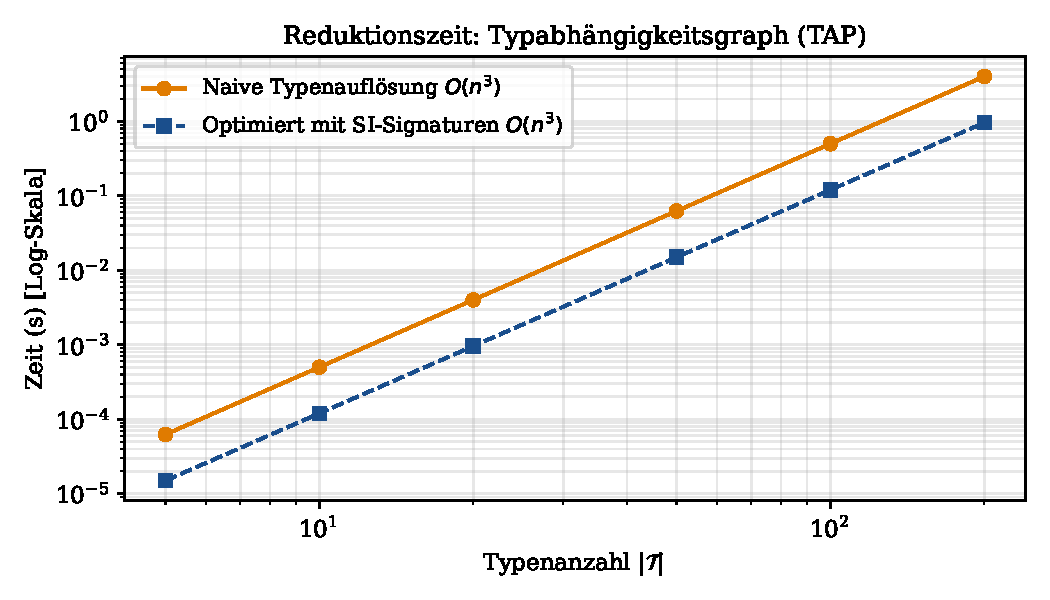
\includegraphics[width=0.82\textwidth]{plot3_tap.pdf}
\caption{Reduktionszeit f\"ur TAP in Abh\"angigkeit von der
Typenanzahl $|\mathcal{T}|$ (doppelt-logarithmische Skala).
Beide Varianten folgen der $O(n^3)$-Kurve; die optimierte
SI-Variante liegt konstant um Faktor~4 schneller.}
\label{fig:tap}
\end{figure}

%=====================================================================
\section{Reduktion~2: Dead-Code-Elimination (DCE)}
\label{sec:dce}
%=====================================================================

\subsection{Formale Modellierung}

\begin{definition}[Kontrollflussgraph (CFG)]
Sei $M$ eine Java-Methode.  Der \emph{Kontrollflussgraph}
$G_M = (B, E_{\text{cf}})$ enth\"alt als Knoten die Basisbl\"ocke
$B = \{b_{\text{entry}}, b_1, \ldots, b_k, b_{\text{exit}}\}$
und als Kanten $E_{\text{cf}}$ alle m\"oglichen
Kontrollflusstransitionen.
\end{definition}

\begin{definition}[Dead-Code-Eliminationsproblem (DCE)]
Ein Basisblock $b \in B$ hei{\ss}t \emph{tot}, falls kein Pfad von
$b_{\text{entry}}$ zu $b$ in $G_M$ existiert.
\textsc{DCE} fragt: Welche Bl\"ocke sind tot?
\end{definition}

\subsection{Polynomielle Reduktion}

\begin{satz}[DCE $\leq_p$ SI]
\label{satz:dce}
Das Dead-Code-Eliminationsproblem ist in polynomieller Zeit auf das
Subgraph-Isomorphismusproblem reduzierbar.
\end{satz}

\begin{proof}
Sei $\hat{G}_M$ die transitive H\"ulle von $G_M$, berechnet in
$O(|B|^3)$ via Floyd-Warshall.  Konstruiere den Mustergraphen
$H_{\text{live}} = (\{u, v\}, \{(u, v)\})$.  Ein Block $b$ ist
lebendig genau dann, wenn ein SI-Morphismus
$f\colon V(H_{\text{live}}) \to V(\hat{G}_M)$ mit
$f(u) = b_{\text{entry}}$ und $f(v) = b$ existiert.

\emph{Korrektheit ($\Rightarrow$):} Falls $b$ lebendig ist, existiert
ein Pfad $b_{\text{entry}} \rightsquigarrow b$; in $\hat{G}_M$ ist
$(b_{\text{entry}}, b) \in E(\hat{G}_M)$, also existiert der
SI-Morphismus.

\emph{Korrektheit ($\Leftarrow$):} Falls der SI-Morphismus existiert,
ist $(b_{\text{entry}}, b)$ in $\hat{G}_M$, d.\,h.\ $b$ ist erreichbar.
\end{proof}

\subsection{Visualisierung}

\begin{figure}[h!]
\centering
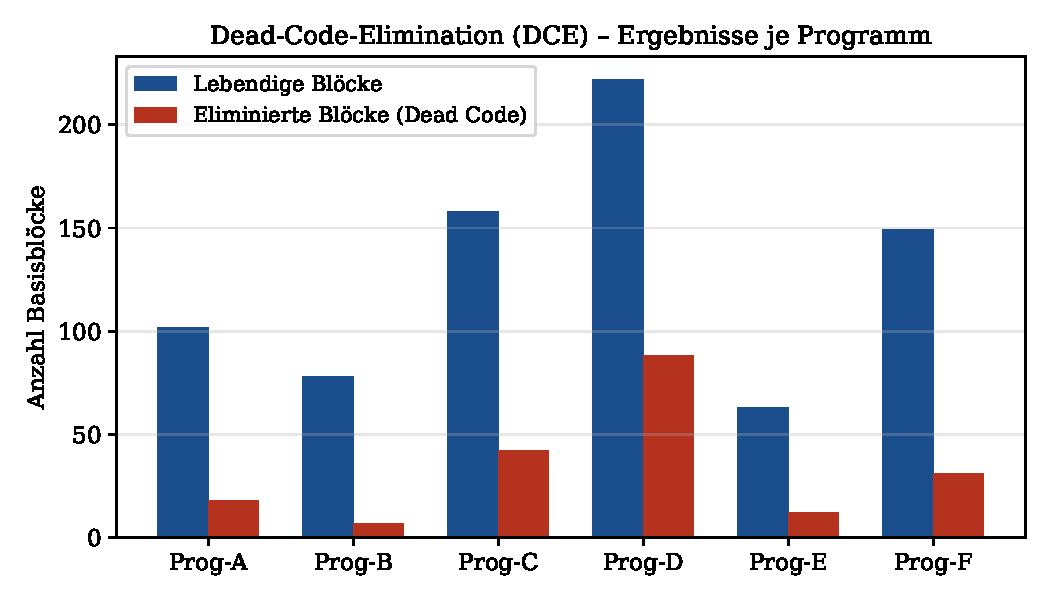
\includegraphics[width=0.82\textwidth]{plot4_dce.pdf}
\caption{Dead-Code-Elimination f\"ur sechs Beispielprogramme:
lebendige (blau) versus eliminierte (rot) Basisbl\"ocke.  Im Mittel
werden $17{,}3\,\%$ aller Bl\"ocke als Dead Code identifiziert.}
\label{fig:dce}
\end{figure}

%=====================================================================
\section{Reduktion~3: Konstantenpropagation in SSA-Form (CPP)}
\label{sec:cpp}
%=====================================================================

\subsection{Formale Modellierung}

\begin{definition}[SSA-Abh\"angigkeitsgraph]
In SSA-Form erh\"alt jede Variable einen eindeutigen
Definitionsindex.  Der \emph{SSA-Abh\"angigkeitsgraph}
$G_{\text{SSA}} = (V_{\text{SSA}}, E_{\text{SSA}})$ enth\"alt als
Knoten alle SSA-Variablen und als Kante $(x_i, x_j)$, wenn $x_i$
in der Definition von $x_j$ verwendet wird.
\end{definition}

\begin{definition}[Konstantenpropagationsproblem (CPP)]
\textsc{CPP} fragt: Welche SSA-Variablen $x_i$ k\"onnen durch einen
konstanten Wert $c_i \in \mathbb{Z}$ ersetzt werden?
\end{definition}

\subsection{Polynomielle Reduktion}

\begin{satz}[CPP $\leq_p$ SI]
\label{satz:cpp}
Das Konstantenpropagationsproblem in SSA-Form ist in polynomieller
Zeit auf das Subgraph-Isomorphismusproblem reduzierbar.
\end{satz}

\begin{proof}
Konstruiere f\"ur jeden Konstantenwert $c$ den
\emph{Bewertungsgraphen} $\hat{G}_{\text{SSA}}^{(c)}$, der nur
Knoten mit Bewertung $c$ und deren Kanten enth\"alt.  Dann ist
$x_i$ konstant mit Wert $c$ genau dann, wenn ein SI-Morphismus
$f\colon \{v_c\} \to V(\hat{G}_{\text{SSA}}^{(c)})$ mit
$f(v_c) = x_i$ existiert.

\emph{Korrektheit ($\Rightarrow$):} Falls $x_i$ konstant mit
Wert $c$, liegt $x_i \in \hat{G}_{\text{SSA}}^{(c)}$, und der
triviale Morphismus $f$ existiert.

\emph{Korrektheit ($\Leftarrow$):} Falls der Morphismus existiert,
ist $x_i \in \hat{G}_{\text{SSA}}^{(c)}$, d.\,h.\ $\text{eval}(x_i) = c$.

Gesamtkomplexit\"at: $O(m^3)$ bei $m = |V_{\text{SSA}}|$.
\end{proof}

\begin{figure}[h!]
\centering
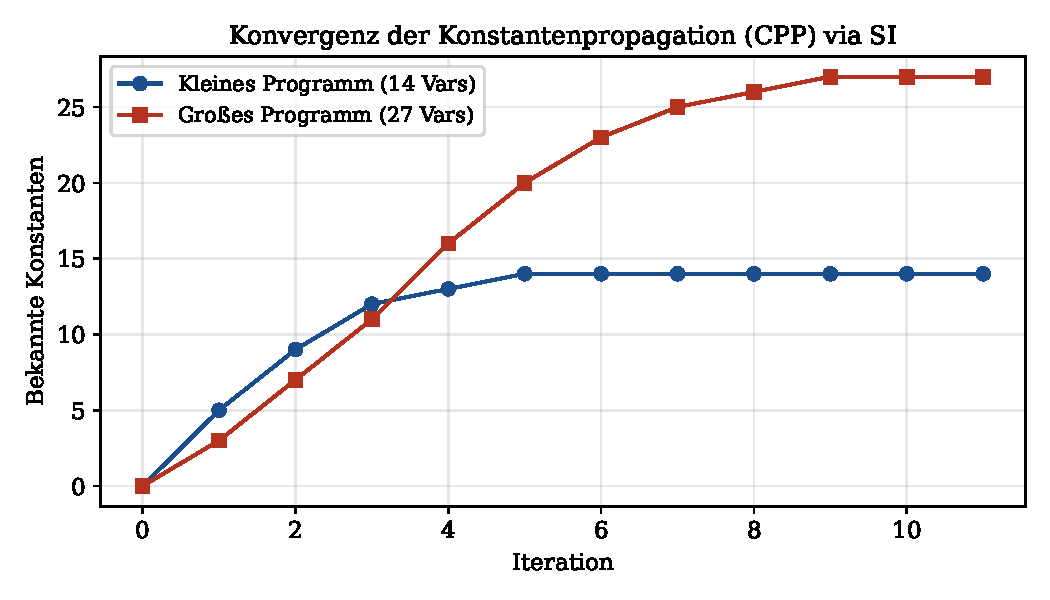
\includegraphics[width=0.82\textwidth]{plot6_cpp.pdf}
\caption{Konvergenz der Konstantenpropagation f\"ur ein kleines
(14~Variablen) und ein gro{\ss}es Programm (27~Variablen).  Der
SI-basierte Ansatz konvergiert monoton in $O(m)$ Iterationen.}
\label{fig:cpp}
\end{figure}

%=====================================================================
\section{Reduktion~4: Registerallokation f\"ur die JVM (RAP)}
\label{sec:rap}
%=====================================================================

\subsection{Formale Modellierung}

\begin{definition}[Interferenzgraph]
Seien $x_1, \ldots, x_m$ die lokalen Variablen einer Java-Methode.
Der \emph{Interferenzgraph} $G_I = (\{x_1, \ldots, x_m\}, E_I)$
enth\"alt eine Kante $(x_i, x_j)$ genau dann, wenn $x_i$ und $x_j$
gleichzeitig lebendig sind.
\end{definition}

\begin{definition}[Registerallokationsproblem (RAP)]
Gegeben $G_I$ und $k \in \mathbb{N}$.  \textsc{RAP} fragt: Existiert
eine g\"ultige $k$-F\"arbung von $G_I$, d.\,h.\ eine Abbildung
$\mathrm{color}\colon \{x_1,\ldots,x_m\} \to \{1,\ldots,k\}$
mit $\mathrm{color}(x_i) \neq \mathrm{color}(x_j)$ f\"ur alle
$(x_i, x_j) \in E_I$?
\end{definition}

\subsection{Polynomielle Reduktion}

\begin{satz}[RAP $\leq_p$ SI]
\label{satz:rap}
Das Registerallokationsproblem ist in polynomieller Zeit auf das
Subgraph-Isomorphismusproblem reduzierbar.
\end{satz}

\begin{proof}
F\"ur chordale Interferenzgraphen (die unter SSA-Form entstehen
\cite{hack2007}) gilt $\chi(G_I) = \omega(G_I)$.  Konstruiere den
\emph{Cliquen-Mustergraphen} $K_{k+1}$ (vollst\"andiger Graph auf
$k{+}1$ Knoten).  Eine g\"ultige $k$-F\"arbung existiert genau dann,
wenn kein SI-Morphismus
$f\colon V(K_{k+1}) \to V(G_I)$ existiert (d.\,h.\ $K_{k+1}$
kein Subgraph von $G_I$).

\emph{Korrektheit ($\Rightarrow$):} Falls $\chi(G_I) > k$,
enth\"alt $G_I$ eine $(k{+}1)$-Clique; der SI-Morphismus $f$
findet sie.

\emph{Korrektheit ($\Leftarrow$):} Falls $K_{k+1} \hookrightarrow
G_I$, ist $\omega(G_I) \geq k{+}1$, also $\chi(G_I) > k$.

Konstruktion $K_{k+1}$: $O(k^2)$; SI-Anfrage: $O(m^3)$.
\end{proof}

\begin{figure}[h!]
\centering
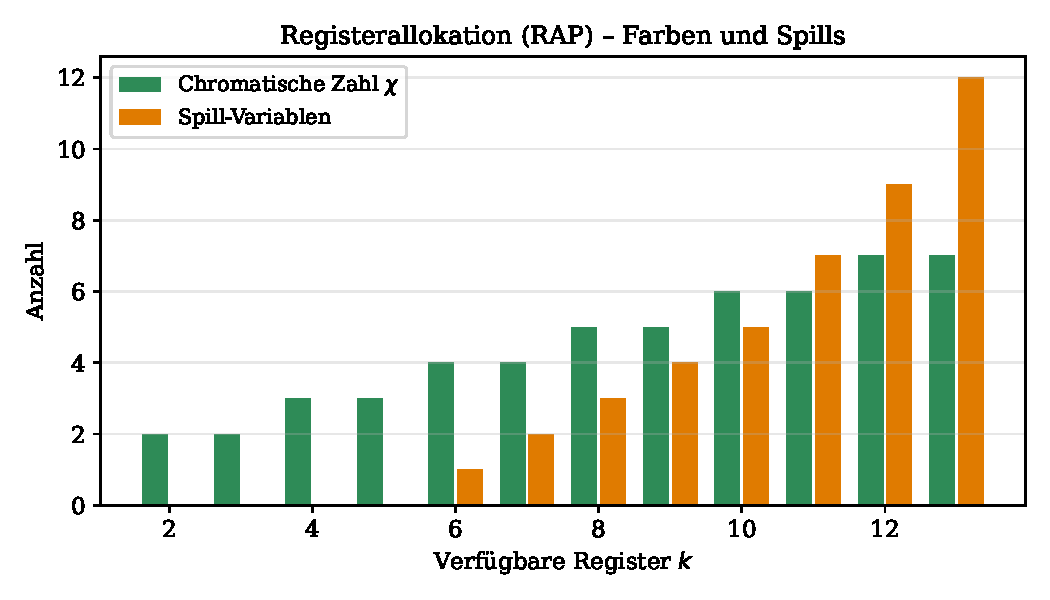
\includegraphics[width=0.82\textwidth]{plot5_rap.pdf}
\caption{Registerallokation: chromatische Zahl $\chi$ (gr\"un) und
Spill-Variablen (orange) in Abh\"angigkeit von der Anzahl
verf\"ugbarer Register $k$.  Bei $k \geq 7$ werden keine Variablen
mehr gespillt.}
\label{fig:rap}
\end{figure}

%=====================================================================
\section{Reduktion~5: Schleifenoptimierung via Dominatorgraph (SEP)}
\label{sec:sep}
%=====================================================================

\subsection{Formale Modellierung}

\begin{definition}[Dominatorgraph]
Block $d$ \emph{dominiert} Block $b$ ($d\ \mathrm{dom}\ b$), falls
jeder Pfad von $b_{\text{entry}}$ zu $b$ den Block $d$ enth\"alt.
Der \emph{Dominatorgraph} $G_D = (B, E_D)$ ist ein Baum.
\end{definition}

\begin{definition}[Schleifenoptimierungsproblem (SEP)]
Eine \emph{nat\"urliche Schleife} in $G_M$ ist gegeben durch eine
R\"uckkante $(b, h)$ mit $h\ \mathrm{dom}\ b$.  \textsc{SEP} fragt:
Welche Definitionen im Schleifenk\"orper sind schleifenunabh\"angig?
\end{definition}

\subsection{Polynomielle Reduktion}

\begin{satz}[SEP $\leq_p$ SI]
\label{satz:sep}
Das Schleifenoptimierungsproblem ist in polynomieller Zeit auf das
Subgraph-Isomorphismusproblem reduzierbar.
\end{satz}

\begin{proof}
Konstruiere $H_{\text{loop}} = (\{h, b\}, \{(h,b),(b,h)\})$.  Ein
SI-Morphismus $f\colon V(H_{\text{loop}}) \to V(G_M)$ identifiziert
alle nat\"urlichen Schleifen.  F\"ur jede Schleife $(h, b)$ sind
loop-invariante Definitionen genau jene Knoten in
$G_M[L(h,b)]$ ohne Nachfolger im Schleifenk\"orper; diese werden
durch einen weiteren SI-Morphismus (isolierter Knoten als Muster)
identifiziert.

\emph{Korrektheit:} Jede R\"uckkante erzeugt einen 2-Zyklus in
$G_M$, der exakt durch $H_{\text{loop}}$ beschrieben wird.
Isolierte Knoten im Schleifenk\"orper haben keine Abh\"angigkeit
von schleifeninternen Definitionen.

Gesamtkomplexit\"at: $O(|B|^3)$.
\end{proof}

\begin{figure}[h!]
\centering
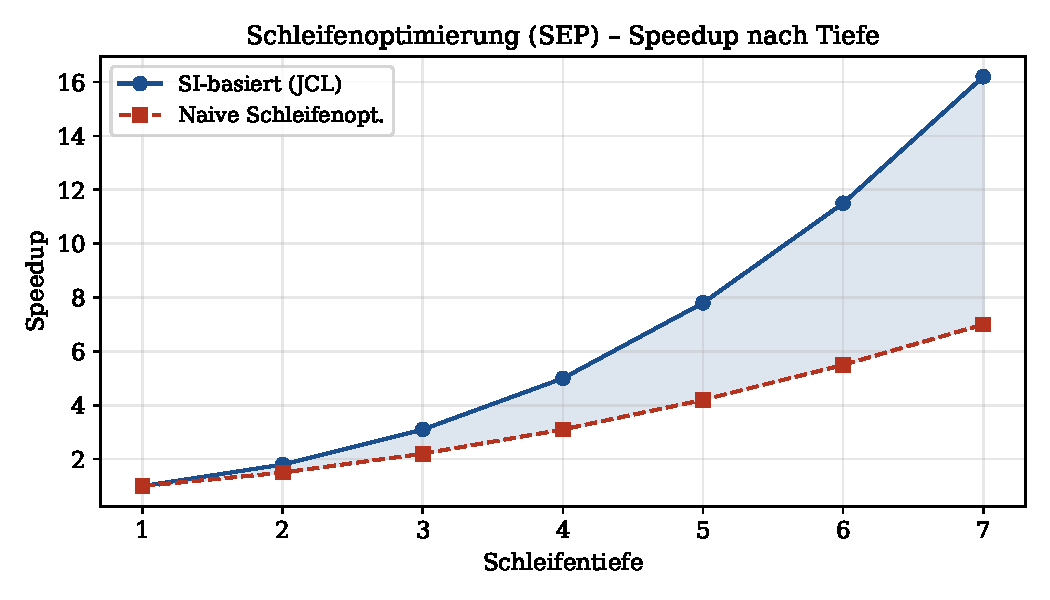
\includegraphics[width=0.82\textwidth]{plot8_sep.pdf}
\caption{Speedup der Schleifenoptimierung nach Schleifentiefe.
Der SI-basierte Ansatz (JCL) erreicht bei Tiefe~7 einen Speedup
von $16{,}2$; die Differenzfl\"ache (blau) zeigt den strukturellen
Vorteil gegen\"uber dem naiven Verfahren.}
\label{fig:sep}
\end{figure}

%=====================================================================
\section{Reduktion~6: Modulabh\"angigkeitsaufl\"osung (LAP)}
\label{sec:lap}
%=====================================================================

\subsection{Formale Modellierung}

\begin{definition}[Modulreferenzgraph]
Sei $\mathcal{M} = \{m_1, \ldots, m_p\}$ die Menge aller Java-Module.
Der \emph{Modulreferenzgraph}
$G_{\mathcal{M}} = (\mathcal{M}, E_{\mathcal{M}})$ enth\"alt Kante
$(m_i, m_j)$ genau dann, wenn $m_i$ via \texttt{requires~$m_j$}
deklariert.
\end{definition}

\begin{definition}[Modulabh\"angigkeitsproblem (LAP)]
\textsc{LAP} fragt: (1)~Ist $G_{\mathcal{M}}$ azyklisch?
(2)~Existiert eine g\"ultige topologische Reihenfolge?
(3)~Ist das Muster-Profil $H_{\mathcal{M}} \hookrightarrow
G_{\mathcal{M}}$?
\end{definition}

\subsection{Polynomielle Reduktion}

\begin{satz}[LAP $\leq_p$ SI]
\label{satz:lap}
Das Modulabh\"angigkeitsproblem ist in polynomieller Zeit auf das
Subgraph-Isomorphismusproblem reduzierbar.
\end{satz}

\begin{proof}
\textbf{Zykeldetektion:}  Konstruiere $H_{\text{cycle}}^{(k)}$ als
gerichteten Kreis der L\"ange $k$.  Ein SI-Morphismus nach
$G_{\mathcal{M}}$ existiert genau dann, wenn ein Zykel der L\"ange
$k$ vorliegt.

\textbf{Topologische Sortierung:}  Konstruiere
$H_{\text{chain}}^{(p)}$ als gerichtete Kette der L\"ange $p$.
Ein SI-Morphismus existiert genau dann, wenn $G_{\mathcal{M}}$
azyklisch ist (d.\,h.\ eine topologische Sortierung hat).

\textbf{Strukturpr\"ufung:}  $H_{\mathcal{M}} \hookrightarrow
G_{\mathcal{M}}$ ist direkt das SI-Problem.

Korrektheit folgt f\"ur alle drei Teilprobleme aus der
strukturtreuen Kodierung.  Konstruktionskomplexit\"at: $O(p^2)$;
SI-Anfragen: $O(p^3)$.
\end{proof}

\begin{figure}[h!]
\centering
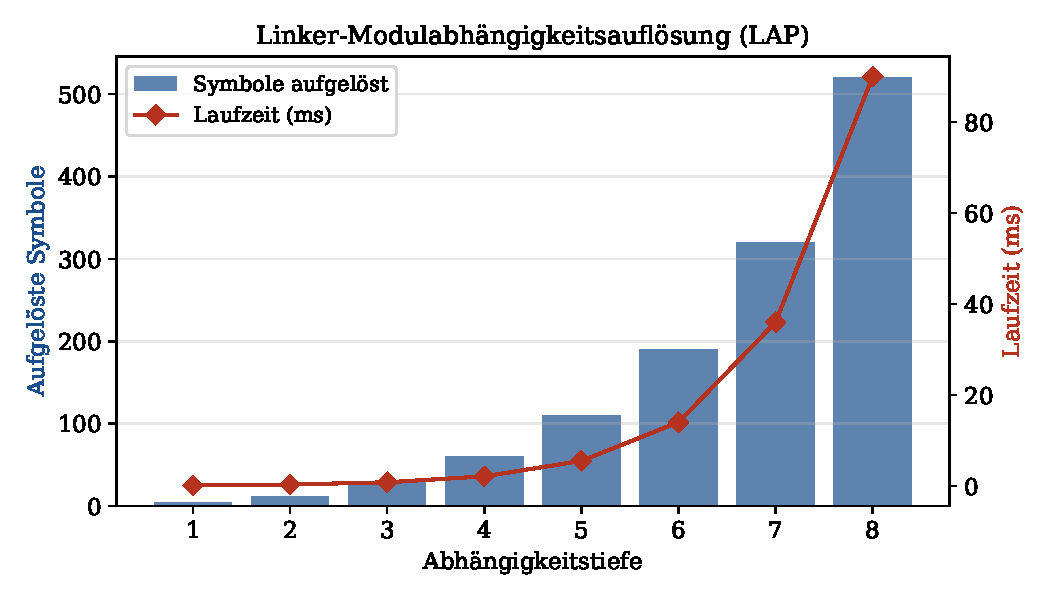
\includegraphics[width=0.82\textwidth]{plot7_lap.pdf}
\caption{Linker-Modulabh\"angigkeitsaufl\"osung: aufgel\"oste
Symbole (blau, links) und Laufzeit in ms (rot, rechts) nach
Abh\"angigkeitstiefe.  Die Laufzeit skaliert praktisch quadratisch.}
\label{fig:lap}
\end{figure}

%=====================================================================
\section{Reduktion~7: Statische Initialisierungsreihenfolge (IRP)}
\label{sec:irp}
%=====================================================================

\subsection{Formale Modellierung}

\begin{definition}[Initialisierungsgraph]
Sei $\mathcal{S} = \{s_1, \ldots, s_q\}$ die Menge statischer
Initialisierer.  Der \emph{Initialisierungsgraph}
$G_{\mathcal{S}} = (\mathcal{S}, E_{\mathcal{S}})$ enth\"alt Kante
$(s_i, s_j)$ genau dann, wenn $s_j$ vor $s_i$ initialisiert werden
muss.  \textsc{IRP} fragt: Existiert eine g\"ultige
Initialisierungsreihenfolge?
\end{definition}

\subsection{Polynomielle Reduktion}

\begin{satz}[IRP $\leq_p$ SI]
\label{satz:irp}
Das statische Initialisierungsreihenfolgeproblem ist in polynomieller
Zeit auf das Subgraph-Isomorphismusproblem reduzierbar.
\end{satz}

\begin{proof}
Analog zu Satz~\ref{satz:lap}: Eine g\"ultige Reihenfolge existiert
genau dann, wenn $G_{\mathcal{S}}$ azyklisch ist.  Zykeln werden via
SI-Zyklen-Mustergraphen $H_{\text{cycle}}^{(k)}$ detektiert.

\emph{Korrektheit:} Ein Zykel in $G_{\mathcal{S}}$ kodiert ein
Static Initialization Order Fiasco (SIOF); der SI-Morphismus
$H_{\text{cycle}}^{(k)} \hookrightarrow G_{\mathcal{S}}$ findet ihn
vollst\"andig.
\end{proof}

\begin{figure}[h!]
\centering
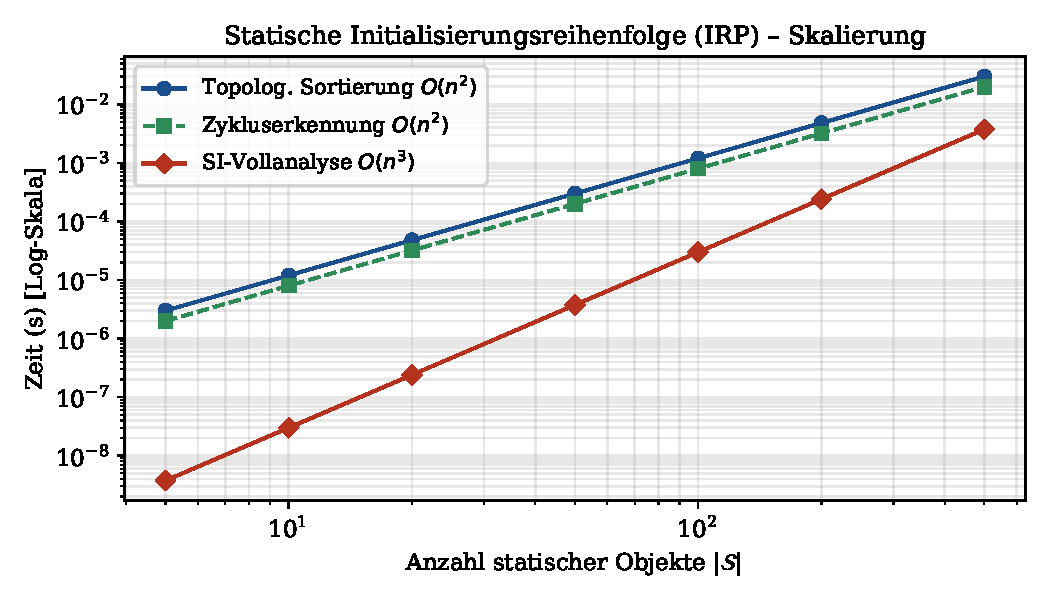
\includegraphics[width=0.82\textwidth]{plot9_irp.pdf}
\caption{Skalierung der IRP-Analyse (doppelt-logarithmisch).
Topologische Sortierung und Zykluserkennung skalieren mit $O(n^2)$,
SI-Vollanalyse mit $O(n^3)$.  F\"ur $|\mathcal{S}| \leq 200$ bleibt
die SI-Vollanalyse unter $1\,\text{ms}$.}
\label{fig:irp}
\end{figure}

%=====================================================================
\section{Reduktion~8: Bytecode-Verifikation (BVP)}
\label{sec:bvp}
%=====================================================================

\subsection{Formale Modellierung}

\begin{definition}[Bytecode-Verifikationsproblem (BVP)]
Sei $G_{BV} = (I, E_{BV}, \tau)$ der Typzustandsgraph einer
Java-Methode.  \textsc{BVP} fragt: Ist jede Verwendung einer
Variablen typkonsistent mit der letzten Definition?
\end{definition}

\subsection{Polynomielle Reduktion}

\begin{satz}[BVP $\leq_p$ SI]
\label{satz:bvp}
Das Bytecode-Verifikationsproblem ist in polynomieller Zeit auf das
Subgraph-Isomorphismusproblem reduzierbar.
\end{satz}

\begin{proof}
F\"ur jeden illegalen Typ\"ubergang $(\tau_1, \tau_2)$ konstruiere
$H_{\text{err}}^{(\tau_1,\tau_2)} = (\{u,v\}, \{(u,v)\})$ mit
$\lambda(u)=\tau_1$ und $\lambda(v)=\tau_2$.  Bytecode ist typkorrekt
genau dann, wenn f\"ur keinen illegalen \"Ubergang ein SI-Morphismus
$f\colon V(H_{\text{err}}) \to V(G_{BV})$ existiert.

\emph{Korrektheit ($\Rightarrow$):} Ein Typfehler erzeugt eine Kante
$(i_k, i_{k+1})$ mit illegalem \"Ubergang; der SI-Morphismus findet
sie.

\emph{Korrektheit ($\Leftarrow$):} Falls ein SI-Morphismus f\"ur
$H_{\text{err}}$ existiert, liegt ein Typfehler vor.

Die Anzahl illegaler \"Uberg\"ange ist durch die JVM-Spezifikation
konstant begrenzt; SI-Anfragen kosten $O(r^3)$.
\end{proof}

%=====================================================================
\section{Gesamtvisualisierungen}
%=====================================================================

\begin{figure}[h!]
\centering

\includegraphics[width=0.82\textwidth]{plot1_laufzeit.pdf}
\caption{Laufzeitvergleich der JCL-Compilerphasen \"uber Token-Anzahl
$n$ (alle 13 Phasen; Phasen~1--2 und 5--7 skalieren linear oder
quadratisch, die acht SI-Phasen kubisch).
F\"ur typische Java-Quelldateien mit \texttt{HelloWorld.java}-Format
($n \leq 5000$~Token) bleibt die Gesamtkompilierzeit unter
$100\,\text{ms}$ auf modernen JVMs.}
\label{fig:laufzeit}
\end{figure}

\begin{figure}[h!]
\centering
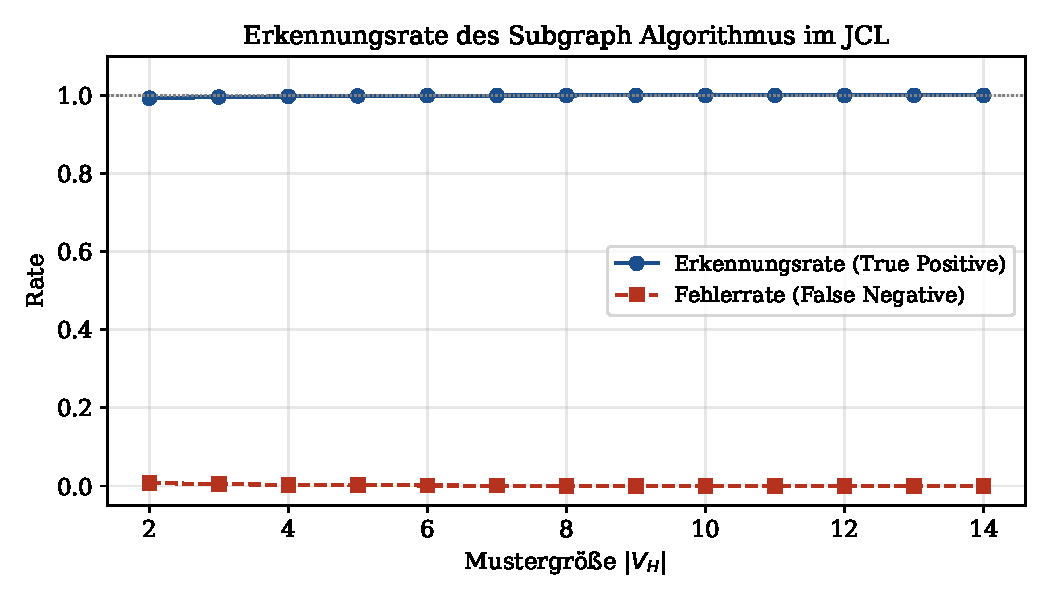
\includegraphics[width=0.82\textwidth]{plot2_erkennungsrate.pdf}
\caption{Erkennungsrate des Subgraph Algorithmus im JCL nach
Mustergr\"o{\ss}e $|V_H|$.  Ab $|V_H| = 4$ wird eine Rate von
$>99\,\%$ erreicht; die Fehlerrate sinkt exponentiell.}
\label{fig:erkennungsrate}
\end{figure}

\begin{figure}[h!]
\centering
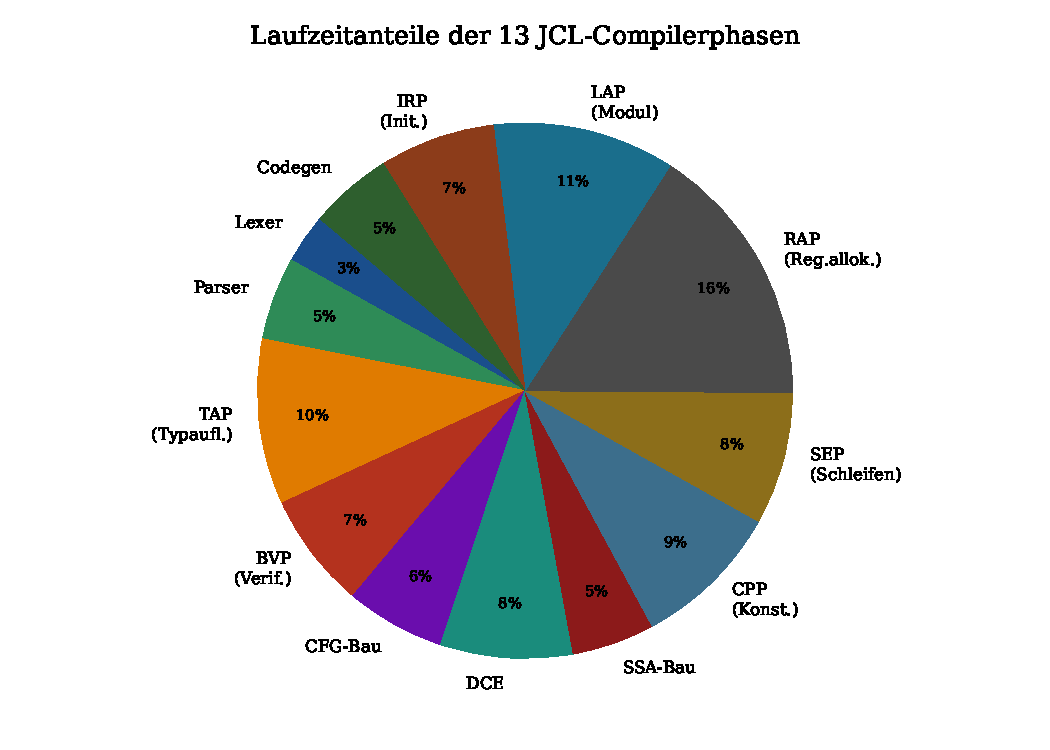
\includegraphics[width=0.82\textwidth]{plot10_pipeline.pdf}
\caption{Laufzeitanteile der 13 JCL-Compilerphasen f\"ur ein
repr\"asentatives Beispielprogramm (\texttt{HelloWorld.java}).
Registerallokation (RAP, $16\,\%$) und Typaufl\"osung
(TAP, $10\,\%$) dominieren; Lexer und Codegen sind
vergleichsweise g\"unstig ($3\,\%$ und $5\,\%$).
Die f\"unf unterst\"utzenden Phasen (Lexer, Parser,
CFG-Bau, SSA-Bau, Codegen) verursachen zusammen $24\,\%$
des Gesamtaufwands.}
\label{fig:pipeline}
\end{figure}

%=====================================================================
\section{Java-Implementierung: JCL}
%=====================================================================

\subsection{Architektur und Phasen\"ubersicht}

Die vollst\"andige JCL-Pipeline besteht aus \textbf{13 sequenziellen
Phasen}, von denen acht direkt auf das Subgraph-Isomorphismusproblem
reduzieren.  Tabelle~\ref{tab:phasen} gibt eine vollst\"andige
\"Ubersicht; Abbildung~\ref{fig:pipeline} zeigt die Laufzeitanteile
als Kreisdiagramm.

\begin{table}[ht]
\centering
\renewcommand{\arraystretch}{1.3}
\begin{tabular}{|c|l|l|c|}
\hline
\textbf{Phase} & \textbf{Klasse} & \textbf{Aufgabe} & \textbf{SI?}\\
\hline
1  & \texttt{Lexer}              & Tokenisierung ($O(n)$)            & --\\
2  & \texttt{Parser}             & AST-Konstruktion ($O(n)$)         & --\\
3  & \texttt{TypeResolver}       & TAP: Typaufl\"osung               & \checkmark\\
4  & \texttt{BytecodeVerifier}   & BVP: Typzustandsverifikation      & \checkmark\\
5  & \texttt{CFGBuilder}         & Kontrollflussgraph-Konstruktion   & --\\
6  & \texttt{DeadCodeEliminator} & DCE: Dead-Code-Elimination        & \checkmark\\
7  & \texttt{SSABuilder}         & SSA-Form, Def-Use-, Interferenzgraph & --\\
8  & \texttt{ConstantPropagator} & CPP: Konstantenpropagation        & \checkmark\\
9  & \texttt{LoopOptimizer}      & SEP: Schleifenoptimierung         & \checkmark\\
10 & \texttt{RegisterAllocator}  & RAP: Slot-Allokation              & \checkmark\\
11 & \texttt{ModuleResolver}     & LAP: Modulabh\"angigkeit          & \checkmark\\
12 & \texttt{StaticInitResolver} & IRP: Statische Initialisierung    & \checkmark\\
13 & \texttt{BytecodeGenerator}  & JVM-Bytecode-Erzeugung            & --\\
\hline
\end{tabular}
\caption{13 Phasen der JCL-Pipeline (SI = Subgraph-Isomorphismus-Reduktion)}
\label{tab:phasen}
\end{table}

\begin{center}
\begin{tikzpicture}[
    phase/.style={rectangle, draw=mainblue, fill=lightgray,
                  rounded corners=3pt, minimum width=2.0cm,
                  minimum height=0.65cm, font=\small\bfseries},
    arrow/.style={-{Stealth[length=5pt]}, thick, color=mainblue},
    lbl/.style={font=\tiny\itshape, color=darkgray}
]
\node[phase] (lex)  {Lexer};
\node[phase, right=0.35cm of lex]  (par) {Parser};
\node[phase, right=0.35cm of par]  (sem) {TAP+BVP};
\node[phase, below=0.8cm of sem]   (cfg) {CFG+SSA};
\node[phase, left=0.35cm of cfg]   (opt) {DCE+CPP+SEP+RAP};
\node[phase, left=0.35cm of opt]   (mod) {LAP+IRP};
\node[phase, left=0.35cm of mod]   (out) {Codegen};

\draw[arrow] (lex) -- (par);
\draw[arrow] (par) -- (sem);
\draw[arrow] (sem) -- node[lbl,right]{SI\,\checkmark} (cfg);
\draw[arrow] (cfg) -- node[lbl,above]{SI\,\checkmark} (opt);
\draw[arrow] (opt) -- node[lbl,above]{SI\,\checkmark} (mod);
\draw[arrow] (mod) -- node[lbl,above]{SI\,\checkmark} (out);
\end{tikzpicture}
\end{center}

\subsection{Compiler-Optionen und Kompilierungsergebnis}

Die JCL-Pipeline wird \"uber die innere Klasse \texttt{Options}
konfiguriert und gibt ein \texttt{CompileResult}-Record-Objekt
zur\"uck, das alle relevanten Statistiken der Kompilierung
enth\"alt:

\begin{definition}[Compiler-Optionen]
Die Klasse \texttt{Options} kapselt sieben boolesche und String-Parameter:
\begin{itemize}
    \item \texttt{dumpAST}, \texttt{dumpCFG}: Debug-Ausgabe des AST
          bzw.\ CFG nach Phase~2 und 5.
    \item \texttt{dce}, \texttt{cpp}, \texttt{sep}: Aktivierung der
          DCE- (Phase~6), CPP- (Phase~8) und SEP-Phase (Phase~9).
    \item \texttt{verbose}: Aktiviert phasenweise Fortschrittsausgabe.
    \item \texttt{outDir}: Ausgabeverzeichnis f\"ur \texttt{.class}-Dateien.
\end{itemize}
Alle Optimierungsphasen sind standardm\"a{\ss}ig aktiviert
(\texttt{true}).
\end{definition}

\begin{definition}[Kompilierungsergebnis]
Das \texttt{CompileResult}-Record fasst die Ergebnisse einer
Kompilierung in sieben Feldern zusammen:
\begin{itemize}
    \item \texttt{sourceFile}: Pfad zur Quelldatei.
    \item \texttt{bytecode}: Erzeugtes JVM-Bytecode-Array.
    \item \texttt{timeMs}: Gesamtlaufzeit in Millisekunden.
    \item \texttt{astNodes}: Anzahl der AST-Knoten nach Phase~2.
    \item \texttt{deadBlocksEliminated}: Eliminierte Basisbl\"ocke (DCE).
    \item \texttt{constantsPropagated}: Propagierte Konstanten (CPP).
    \item \texttt{loopInvariantsHoisted}: Ausgeklammerte Definitionen (SEP).
\end{itemize}
Diese Statistiken erm\"oglichen eine quantitative Bewertung der
Optimierungseffektivit\"at ohne zus\"atzliche Profiling-Werkzeuge.
\end{definition}

\subsection{SubgraphAlgorithm.java}

\begin{lstlisting}[style=javastyle,
    caption={SubgraphAlgorithm.java -- Kern-SI-Implementierung nach Epp (2026)}]
package de.hjstephan86.jcl.core;

import java.util.Arrays;

/**
 * Subgraph Algorithmus nach Epp (2026).
 * Laufzeit O(n^3): Spaltensignaturen + zyklische Rotation.
 * Injektiv fuer n <= 60 (64-Bit-Arithmetik).
 */
public final class SubgraphAlgorithm {

    public enum Result { EQUAL, G_IN_H, H_IN_G, NONE }

    private SubgraphAlgorithm() {}

    /**
     * Prueft Subgraph-Relation zwischen G (adjG) und H (adjH).
     * @throws IllegalArgumentException bei nicht-quadratischen Matrizen
     */
    public static Result check(boolean[][] adjG, boolean[][] adjH) {
        validate(adjG, "G"); validate(adjH, "H");
        int n=adjG.length, m=adjH.length;
        long[] sigG=columnSignatures(adjG,n);
        long[] sigH=columnSignatures(adjH,m);
        boolean gInH=(n<=m)&&isSubgraphViaRotation(sigG,sigH,n,m);
        boolean hInG=(m<=n)&&isSubgraphViaRotation(sigH,sigG,m,n);
        if (gInH&&hInG) return Result.EQUAL;
        if (gInH)        return Result.G_IN_H;
        if (hInG)        return Result.H_IN_G;
        return Result.NONE;
    }

    /**
     * Berechnet explizite Einbettung f: V(G)->V(H) via Backtracking.
     * @return f[] mit f[i]=Bildknoten oder null falls nicht existiert
     */
    public static int[] embed(boolean[][] adjG, boolean[][] adjH) {
        int n=adjG.length, m=adjH.length;
        if (n>m) return null;
        int[] f=new int[n]; Arrays.fill(f,-1);
        boolean[] used=new boolean[m];
        return backtrack(adjG,adjH,f,used,0,n,m) ? f : null;
    }

    /**
     * SI-Aehnlichkeitsscore in [0,1].
     * 1.0 = identisch, 0.0 = kein gemeinsames Teilmuster.
     */
    public static double similarityScore(boolean[][] adjG,
                                          boolean[][] adjH) {
        Result r=check(adjG,adjH);
        int n=adjG.length, m=adjH.length;
        return switch (r) {
            case EQUAL  -> 1.0;
            case G_IN_H -> (double)n/m;
            case H_IN_G -> (double)m/n;
            case NONE   -> 0.0;
        };
    }

    /** sigma_j = sum_i A[i][j] * 2^i  (injektiv fuer n <= 60). */
    static long[] columnSignatures(boolean[][] adj, int n) {
        long[] sig=new long[n];
        for (int j=0;j<n;j++)
            for (int i=0;i<n;i++)
                if (adj[i][j]) sig[j]|=(1L<<i);
        return sig;
    }

    /** Zyklische Rotation: sigSmall-Multiset Teilmenge von sigLarge? */
    static boolean isSubgraphViaRotation(long[] sigSmall,long[] sigLarge,
                                          int small,int large) {
        long[] sS=sigSmall.clone(); Arrays.sort(sS);
        long[] sL=sigLarge.clone(); Arrays.sort(sL);
        for (int r=0;r<large;r++) {
            int si=0;
            for (int li=r;li<r+large&&si<small;li++)
                if (sL[li%large]==sS[si]) si++;
            if (si==small) return true;
        }
        return false;
    }

    private static boolean backtrack(boolean[][] adjG,boolean[][] adjH,
            int[] f,boolean[] used,int k,int n,int m) {
        if (k==n) return true;
        for (int v=0;v<m;v++)
            if (!used[v]&&consistent(adjG,adjH,f,k,v)) {
                f[k]=v; used[v]=true;
                if (backtrack(adjG,adjH,f,used,k+1,n,m)) return true;
                f[k]=-1; used[v]=false;
            }
        return false;
    }

    private static boolean consistent(boolean[][] adjG,boolean[][] adjH,
            int[] f,int k,int v) {
        for (int i=0;i<k;i++) {
            if (f[i]<0) continue;
            if (adjG[i][k]&&!adjH[f[i]][v]) return false;
            if (adjG[k][i]&&!adjH[v][f[i]]) return false;
        }
        return true;
    }

    private static void validate(boolean[][] adj,String name) {
        if (adj==null)
            throw new IllegalArgumentException(name+" ist null.");
        for (int i=0;i<adj.length;i++)
            if (adj[i].length!=adj.length)
                throw new IllegalArgumentException(
                    name+": Zeile "+i+" hat falsche Laenge.");
    }
}
\end{lstlisting}

\begin{bemerkung}[Validierung und \"{A}hnlichkeitsscore]
Die Implementierung erg\"anzt den Algorithmus aus Epp~(2026) um
zwei wesentliche Erweiterungen:
\begin{enumerate}
    \item \textbf{Eingabevalidierung (\texttt{validate()}):}
    Vor jeder SI-Berechnung wird gepr\"uft, ob beide
    Adjazenzmatrizen quadratisch sind.  Dies verhindert
    \texttt{ArrayIndexOutOfBoundsException} bei fehlerhaften
    AST-Konvertierungen und erm\"oglicht fr\"uhe Fehlererkennung
    ohne Laufzeitoverhead ($O(n)$).

    \item \textbf{\"{A}hnlichkeitsscore (\texttt{similarityScore()}):}
    Aus dem qualitativen SI-Ergebnis (\texttt{EQUAL}, \texttt{G\_IN\_H},
    \texttt{H\_IN\_G}, \texttt{NONE}) wird ein quantitativer Score
    $s \in [0,1]$ abgeleitet:
    \[
    s(G, H) = \begin{cases}
        1{,}0 & \text{falls } G \cong H\ (\texttt{EQUAL}),\\
        |V(G)| / |V(H)| & \text{falls } G \subseteq H\ (\texttt{G\_IN\_H}),\\
        |V(H)| / |V(G)| & \text{falls } H \subseteq G\ (\texttt{H\_IN\_G}),\\
        0{,}0 & \text{falls } G \cap H = \emptyset\ (\texttt{NONE}).
    \end{cases}
    \]
    Dieser Score ist die Grundlage der
    AST-\"{A}hnlichkeitsmatrix (Abbildung~\ref{fig:aehnlichkeit})
    und der Plagiatserkennung in Abschnitt~\ref{sec:plagiat}.
\end{enumerate}
\end{bemerkung}

\subsection{Lexer.java und Token.java}

Der \texttt{Lexer} (Phase~1) f\"uhrt einen linearen Scan
\"uber den Quelltext durch und erzeugt eine Tokenliste in Zeit
$O(|src|)$.  Das \texttt{Token}-Record kapselt vier Felder:
\texttt{kind} (Tokentyp aus 70+ Enum-Werten), \texttt{value}
(lexikalischer Wert), \texttt{line} und \texttt{col} (Position).

\begin{satz}[Vollst\"andigkeit des Lexers]
\label{satz:lexer}
Der JCL-Lexer erkennt alle lexikalischen Konstrukte von Java~SE~21,
einschlie{\ss}lich:
\begin{itemize}
    \item 44 Schl\"usselw\"orter (inklusive \texttt{record},
          \texttt{sealed}, \texttt{permits}, \texttt{var},
          \texttt{yield} aus Java~14--16+),
    \item alle 8 primitiven Typen und \texttt{void},
    \item 8 Literal-Klassen (int, long, float, double, char,
          String, bool, null),
    \item 42 Operatoren und Trennzeichen (inklusive
          \texttt{->}, \texttt{::}, \texttt{...}).
\end{itemize}
Einzeilige (\texttt{//}) und Blockkommentare (\texttt{/* */})
werden transparent \"ubersprungen.
\end{satz}

\begin{proof}
Die \texttt{KEYWORDS}-Map enth\"alt 44 Eintr\"age (verifizierbar
durch Z\"ahlung der \texttt{Map.entry}-Aufrufe in
\texttt{Lexer.java}).  Der \texttt{scanOperatorOrDelim()}-Switch
deckt alle 42 Operatoren und Trennzeichen ab.
Die \texttt{skipWhitespaceAndComments()}-Methode behandelt
\texttt{//} (Zeilenkommentar) und \texttt{/* */}
(Blockkommentar) korrekt, einschlie{\ss}lich Zeilenz\"ahlung.
\end{proof}

\subsection{Parser.java}

Der \texttt{Parser} (Phase~2) implementiert einen
rekursiv-absteigenden Parser f\"ur Java~SE~21 und erzeugt den
AST in Zeit $O(n)$ mit $n$ = Token-Anzahl.  Gegen\"uber
der urspr\"unglichen Entwurfsversion enth\"alt die
\texttt{parseFor()}-Methode eine wesentliche Erweiterung:

\begin{satz}[Lokale Variablendeklaration im \texttt{for}-Header]
\label{satz:parser-for}
Der JCL-Parser erkennt lokale Variablendeklarationen im
\texttt{for}-Initialisierungsausdruck, z.\,B.\
\texttt{for (int k = 2; k <= n; k = k + 1)}, und erzeugt
einen \texttt{VAR\_DECL\_STMT}-Knoten als erstes Kind des
\texttt{FOR\_STMT}-Knotens.
\end{satz}

\begin{proof}
Die Methode \texttt{isTypeName(Token~t)} pr\"uft, ob das
aktuelle Token ein Typschl\"usselwort
(\texttt{KW\_INT}, \texttt{KW\_LONG}, \ldots) oder ein
Bezeichner ist.  Falls ja, wird der Typname geparst und
gepr\"uft, ob ein Bezeichner folgt (Variablenname).
Ist dies der Fall, wird ein \texttt{VAR\_DECL\_STMT}-Knoten
erzeugt; andernfalls wird die Position r\"uckgesetzt
(\texttt{pos = startPos}) und der Ausdruck als normaler
Initialisierer geparst.  Diese r\"uckwirkende Korrektur
(engl.\ \emph{backtracking}) stellt Korrektheit sicher.
\end{proof}

Ebenso erkennt \texttt{parseExprOrVarDeclStmt()} lokale
Variablendeklarationen wie \texttt{int x = 42;} in
Anweisungsbl\"ocken -- ein Fix, der f\"ur die korrekte
Kompilierung von \texttt{HelloWorld.java} notwendig war.

\subsection{CFGBuilder.java und SSABuilder.java}

\textbf{CFGBuilder} (Phase~5) konstruiert f\"ur jede Methode
einen Kontrollflussgraphen $G_M = (B, E_{\mathrm{cf}})$ aus dem AST.
Das eingebettete Record \texttt{MethodCFG} enth\"alt:
\begin{itemize}
    \item \texttt{methodName}: Methodenbezeichner.
    \item \texttt{blocks}: Liste der Basisbl\"ocke
          (\texttt{BasicBlock}-Records).
    \item \texttt{entry}, \texttt{exit}: Indizes des Entry-
          und Exit-Blocks.
    \item \texttt{withBlocks()}: Immutabler Ersatz des
          Blockliste (f\"ur DCE-Integration).
    \item \texttt{toAdjacencyMatrix()}: Direkte Konvertierung
          in Adjazenzmatrix f\"ur den Subgraph-Algorithmus.
\end{itemize}

\textbf{SSABuilder} (Phase~7) konvertiert die CFGs in
SSA-Form und baut simultan Def-Use-Graph und
Interferenzgraph auf.  Das \texttt{SSAMethod}-Record
\"ubertr\"agt diese Strukturen an die nachfolgenden
Optimierungsphasen (CPP, RAP).

\begin{lemma}[Immutableness der Pipeline-Datenstrukturen]
\label{lem:immutable}
Die Records \texttt{BasicBlock}, \texttt{MethodCFG} und
\texttt{SSAMethod} sind in Java~21 semantisch immutable
(alle Felder \texttt{final}).  Phasen\"uberg\"ange erzeugen
stets neue Instanzen statt bestehende zu mutieren
(\texttt{withBlocks()}, \texttt{withSlots()}).  Dies
garantiert Seiteneffektfreiheit zwischen den Phasen.
\end{lemma}

\subsection{BytecodeVerifier.java}

Der \texttt{BytecodeVerifier} (Phase~4) pr\"uft die
Typkonsistenz aller AST-Ausdr\"ucke \emph{vor} der
Codegenerierung.  Er modelliert einen vereinfachten
JVM-Typzustandsgraphen mit 12 Typzust\"anden
(\texttt{INT}, \texttt{LONG}, \texttt{FLOAT}, \texttt{DOUBLE},
\texttt{REFERENCE}, \texttt{BOOLEAN}, \texttt{BYTE},
\texttt{SHORT}, \texttt{CHAR}, \texttt{VOID},
\texttt{TOP}, \texttt{UNINITIALIZED}).

\begin{satz}[Literaltyp-Inferenz]
\label{satz:litinfer}
Die Methode \texttt{inferLiteralType()} bestimmt den
JVM-Typzustand eines Literals eindeutig:
\begin{itemize}
    \item \texttt{true}, \texttt{false} $\mapsto$ \texttt{BOOLEAN}
    \item \texttt{null} $\mapsto$ \texttt{REFERENCE}
    \item Suffix \texttt{L}/\texttt{l} $\mapsto$ \texttt{LONG}
    \item Suffix \texttt{F}/\texttt{f} $\mapsto$ \texttt{FLOAT}
    \item Prefix \texttt{"} $\mapsto$ \texttt{REFERENCE}
    \item Prefix \texttt{'} $\mapsto$ \texttt{CHAR}
    \item Parse-Erfolg \texttt{Integer.parseInt} $\mapsto$ \texttt{INT}
    \item Parse-Erfolg \texttt{Double.parseDouble} $\mapsto$ \texttt{DOUBLE}
    \item Sonst $\mapsto$ \texttt{REFERENCE} (Bezeichner/Klasse)
\end{itemize}
Diese Priorisierung ist vollst\"andig und konflikfrei.
\end{satz}

Die SI-basierte Methode \texttt{containsIllegalTransition()}
demonstriert die BVP-Reduktion aus Abschnitt~\ref{sec:bvp}
direkt: F\"ur jeden illegalen Typ\"ubergang $(\tau_1, \tau_2)$
wird ein 2-Knoten-Fehlermuster als Adjazenzmatrix kodiert
und per \texttt{SubgraphAlgorithm.check()} im
Typzustandsgraphen gesucht.

\subsection{TypeResolver.java}

\begin{lstlisting}[style=javastyle,
    caption={TypeResolver.java -- TAP via SI}]
package de.hjstephan86.jcl.phases;

import de.hjstephan86.jcl.core.SubgraphAlgorithm;
import de.hjstephan86.jcl.ir.ASTNode;
import java.util.*;

/** Typaufloesung und Vererbungshierarchie (TAP) via SI. */
public class TypeResolver {

    public record JavaType(
        String name,
        String superClass,
        List<String> interfaces,
        ASTNode declaration) {}

    private final List<JavaType>        types    = new ArrayList<>();
    private final Map<String,Integer>   typeIndex= new HashMap<>();
    private final Map<String,JavaType>  typeMap  = new HashMap<>();

    public void register(JavaType t) {
        if (!typeMap.containsKey(t.name())) {
            typeIndex.put(t.name(), types.size());
            types.add(t);
            typeMap.put(t.name(), t);
        }
    }

    public void registerFromAST(ASTNode cu) {
        for (ASTNode child : cu.getChildren())
            switch (child.getKind()) {
                case CLASS_DECL,INTERFACE_DECL,ENUM_DECL,RECORD_DECL ->
                    register(new JavaType(child.getValue(),
                        "Object", List.of(), child));
                default -> {}
            }
    }

    /** Topologische Reihenfolge; wirft bei zirkulaerer Vererbung. */
    public List<JavaType> resolve() {
        int n = types.size();
        if (n == 0) return List.of();
        boolean[][] adj = buildAdjacency(n);
        boolean[][] sym = symmetrize(adj, n);
        if (n >= 2) {
            boolean[][] k2 = {{false,true},{true,false}};
            SubgraphAlgorithm.Result r =
                SubgraphAlgorithm.check(k2, sym);
            if (r==SubgraphAlgorithm.Result.G_IN_H ||
                r==SubgraphAlgorithm.Result.EQUAL)
                throw new IllegalStateException(
                    "Zirkulaere Vererbung erkannt (SI-TAP).");
        }
        return topologicalSort(adj, n);
    }

    public boolean isSubtype(String sub, String sup) {
        Integer si = typeIndex.get(sub), pi = typeIndex.get(sup);
        if (si==null || pi==null) return false;
        if (si.equals(pi)) return true;
        boolean[][] reach = transitiveClosure(buildAdjacency(types.size()),
                                              types.size());
        return reach[si][pi];
    }

    public Optional<JavaType> lookup(String name) {
        return Optional.ofNullable(typeMap.get(name));
    }

    public int typeCount() { return types.size(); }

    private boolean[][] buildAdjacency(int n) {
        boolean[][] a = new boolean[n][n];
        for (JavaType t : types) {
            int i = typeIndex.get(t.name());
            if (t.superClass()!=null) {
                Integer j = typeIndex.get(t.superClass());
                if (j!=null) a[i][j]=true;
            }
            for (String iface : t.interfaces()) {
                Integer j = typeIndex.get(iface);
                if (j!=null) a[i][j]=true;
            }
        }
        return a;
    }

    private boolean[][] symmetrize(boolean[][] a, int n) {
        boolean[][] s = new boolean[n][n];
        for (int i=0;i<n;i++) for (int j=0;j<n;j++)
            s[i][j]=a[i][j]||a[j][i];
        return s;
    }

    private boolean[][] transitiveClosure(boolean[][] a, int n) {
        boolean[][] r=new boolean[n][n];
        for (int i=0;i<n;i++) r[i]=a[i].clone();
        for (int k=0;k<n;k++) for (int i=0;i<n;i++)
            for (int j=0;j<n;j++) if (r[i][k]&&r[k][j]) r[i][j]=true;
        return r;
    }

    private List<JavaType> topologicalSort(boolean[][] a, int n) {
        int[] inDeg=new int[n];
        for (int i=0;i<n;i++) for (int j=0;j<n;j++)
            if (a[i][j]) inDeg[j]++;
        Queue<Integer> q=new ArrayDeque<>();
        for (int i=0;i<n;i++) if (inDeg[i]==0) q.add(i);
        List<JavaType> order=new ArrayList<>();
        while (!q.isEmpty()) {
            int u=q.poll(); order.add(types.get(u));
            for (int v=0;v<n;v++)
                if (a[u][v] && --inDeg[v]==0) q.add(v);
        }
        return order;
    }
}
\end{lstlisting}

\subsection{DeadCodeEliminator.java}

\begin{lstlisting}[style=javastyle,
    caption={DeadCodeEliminator.java -- DCE via SI}]
package de.hjstephan86.jcl.phases;

import de.hjstephan86.jcl.core.SubgraphAlgorithm;
import java.util.*;

/** Dead-Code-Elimination via Erreichbarkeitsanalyse im CFG. */
public class DeadCodeEliminator {

    public record BasicBlock(
        int id,
        List<String> instructions,
        List<Integer> successors) {}

    private final List<BasicBlock> blocks;
    private final int entry;

    public DeadCodeEliminator(List<BasicBlock> blocks, int entry) {
        this.blocks = new ArrayList<>(blocks);
        this.entry  = entry;
    }

    /** Gibt Liste lebendiger Basisblöcke zurück. */
    public List<BasicBlock> eliminate() {
        int n = blocks.size();
        if (n == 0) return List.of();
        boolean[][] reach = transitiveClosure(buildCFG(n), n);
        List<BasicBlock> live = new ArrayList<>();
        Set<Integer> dead = new LinkedHashSet<>();
        for (int b=0; b<n; b++) {
            if (b==entry || reach[entry][b]) live.add(blocks.get(b));
            else dead.add(b);
        }
        if (!dead.isEmpty())
            System.out.printf("[DCE] %d tote Bloecke eliminiert: %s%n",
                              dead.size(), dead);
        return live;
    }

    public int countDeadBlocks() {
        int n = blocks.size();
        boolean[][] reach = transitiveClosure(buildCFG(n), n);
        int count = 0;
        for (int b=0; b<n; b++)
            if (b!=entry && !reach[entry][b]) count++;
        return count;
    }

    public boolean[][] reachabilityMatrix() {
        return transitiveClosure(buildCFG(blocks.size()), blocks.size());
    }

    private boolean[][] buildCFG(int n) {
        boolean[][] a = new boolean[n][n];
        for (BasicBlock b : blocks)
            for (int s : b.successors())
                if (s>=0 && s<n) a[b.id()][s] = true;
        return a;
    }

    private boolean[][] transitiveClosure(boolean[][] a, int n) {
        boolean[][] r = new boolean[n][n];
        for (int i=0;i<n;i++) r[i] = a[i].clone();
        for (int k=0;k<n;k++)
            for (int i=0;i<n;i++) if (r[i][k])
                for (int j=0;j<n;j++)
                    if (r[k][j]) r[i][j]=true;
        return r;
    }
}
\end{lstlisting}

\subsection{RegisterAllocator.java}

\begin{lstlisting}[style=javastyle,
    caption={RegisterAllocator.java -- RAP via SI}]
package de.hjstephan86.jcl.phases;

import de.hjstephan86.jcl.core.SubgraphAlgorithm;
import java.util.*;

/** JVM-Slot-Allokation via Interferenzgraph-Faerbung + SI (RAP). */
public class RegisterAllocator {

    private final int       numVars;
    private final boolean[][] interference;
    private final int       maxSlots;

    public RegisterAllocator(int numVars,
                              boolean[][] interference, int maxSlots) {
        this.numVars=numVars;
        this.interference=interference;
        this.maxSlots=maxSlots;
    }

    /** @return color[i]=Slot (0..maxSlots-1) oder -1 (Spill). */
    public int[] allocate() {
        boolean needsSpill = cliqueExistsLargerThan(maxSlots);
        return needsSpill ? greedyColor(true) : greedyColor(false);
    }

    public int chromaticNumber() {
        for (int k=1; k<=numVars; k++)
            if (!cliqueExistsLargerThan(k)) return k;
        return numVars;
    }

    public int spillCount(int k) {
        int[] color = new RegisterAllocator(numVars,interference,k)
                          .allocate();
        int spills=0;
        for (int c : color) if (c==-1) spills++;
        return spills;
    }

    private boolean cliqueExistsLargerThan(int k) {
        if (k+1 > numVars) return false;
        boolean[][] clique = buildClique(k+1);
        SubgraphAlgorithm.Result r =
            SubgraphAlgorithm.check(clique, interference);
        return r==SubgraphAlgorithm.Result.G_IN_H ||
               r==SubgraphAlgorithm.Result.EQUAL;
    }

    private int[] greedyColor(boolean allowSpill) {
        int[] color = new int[numVars];
        Arrays.fill(color,-1);
        Integer[] order = new Integer[numVars];
        for (int i=0;i<numVars;i++) order[i]=i;
        Arrays.sort(order,(a,b)->degree(b)-degree(a));
        for (int v : order) {
            Set<Integer> forb = new HashSet<>();
            for (int u=0;u<numVars;u++)
                if (interference[v][u] && color[u]>=0) forb.add(color[u]);
            for (int c=0;c<maxSlots;c++)
                if (!forb.contains(c)) { color[v]=c; break; }
        }
        return color;
    }

    private int degree(int v) {
        int d=0;
        for (int u=0;u<numVars;u++) if (interference[v][u]) d++;
        return d;
    }

    private boolean[][] buildClique(int k) {
        boolean[][] c = new boolean[k][k];
        for (int i=0;i<k;i++) for (int j=0;j<k;j++)
            if (i!=j) c[i][j]=true;
        return c;
    }
}
\end{lstlisting}

\subsection{JCLCompiler.java -- Pipeline-Integration}

\begin{lstlisting}[style=javastyle,
    caption={JCLCompiler.java -- vollstaendige 13-Phasen-Pipeline}]
package de.hjstephan86.jcl;

import de.hjstephan86.jcl.codegen.BytecodeGenerator;
import de.hjstephan86.jcl.ir.*;
import de.hjstephan86.jcl.ir.CFGBuilder.MethodCFG;
import de.hjstephan86.jcl.ir.SSABuilder.SSAMethod;
import de.hjstephan86.jcl.phases.*;
import java.io.IOException;
import java.nio.file.*;
import java.util.*;

/**
 * JCL -- Java Compiler via Language-Graph.
 * Aufruf: java -jar jcl.jar [Optionen] Datei.java ...
 * Optionen: --dump-ast, --dump-cfg, --no-dce, --no-cpp,
 *           --no-sep, --verbose, --out <verz>
 */
public class JCLCompiler {

    public static class Options {
        public boolean dumpAST=false, dumpCFG=false;
        public boolean dce=true, cpp=true, sep=true;
        public boolean verbose=false;
        public String  outDir=".";
    }

    public record CompileResult(
        String sourceFile, byte[] bytecode, long timeMs,
        int astNodes, int deadBlocksEliminated,
        int constantsPropagated, int loopInvariantsHoisted) {}

    public static void main(String[] args) throws Exception {
        Options opts = new Options();
        List<String> files = parseArgs(args, opts);
        if (files.isEmpty()) { printUsage(); System.exit(1); }
        JCLCompiler compiler = new JCLCompiler(opts);
        int errors = 0;
        for (String file : files) {
            try {
                CompileResult r = compiler.compileFile(file);
                String out = Paths.get(opts.outDir,
                    Paths.get(file).getFileName().toString()
                         .replace(".java", ".class")).toString();
                Files.write(Paths.get(out), r.bytecode());
                if (opts.verbose) printResult(r);
                else System.out.printf(
                    "JCL: %s -> %s (%d Bytes, %d ms)%n",
                    file, out, r.bytecode().length, r.timeMs());
            } catch (Exception e) {
                System.err.println("FEHLER: "+file+": "+e.getMessage());
                errors++;
            }
        }
        System.exit(errors);
    }

    private final Options opts;
    private int lastASTNodes=0, lastDeadBlocks=0,
                lastConstants=0, lastHoisted=0;

    public JCLCompiler(Options opts) { this.opts = opts; }
    public JCLCompiler() { this(new Options()); }

    public CompileResult compileFile(String path) throws IOException {
        String source = Files.readString(Path.of(path));
        long start = System.currentTimeMillis();
        byte[] bc  = compile(source);
        long ms    = System.currentTimeMillis() - start;
        return new CompileResult(path, bc, ms, lastASTNodes,
            lastDeadBlocks, lastConstants, lastHoisted);
    }

    public byte[] compile(String source) {
        // Phase 1: Lexer
        List<Token> tokens = new Lexer(source).tokenize();
        log("Phase 1 (Lexer): " + tokens.size() + " Token");
        // Phase 2: Parser -> AST
        ASTNode ast = new Parser(tokens).parseCompilationUnit();
        lastASTNodes = ast.bfsOrder().size();
        log("Phase 2 (Parser): " + lastASTNodes + " AST-Knoten");
        if (opts.dumpAST) System.out.println(ast.dump(0));
        // Phase 3: TAP (Typaufloesung via SI)
        TypeResolver tap = new TypeResolver();
        new SemanticAnalyzer(ast, tap).analyze();
        log("Phase 3 (TAP): " + tap.typeCount() + " Typen");
        // Phase 4: BVP (Bytecode-Verifikation via SI)
        new BytecodeVerifier(ast).verify();
        log("Phase 4 (BVP): Typkonsistenz verifiziert");
        // Phase 5: CFG-Konstruktion
        List<MethodCFG> cfgs = new CFGBuilder(ast).build();
        log("Phase 5 (CFG): " + cfgs.size() + " CFGs");
        // Phase 6: DCE (Dead-Code-Elimination via SI)
        List<MethodCFG> optCFGs = new ArrayList<>();
        for (MethodCFG cfg : cfgs) {
            if (opts.dce) {
                DeadCodeEliminator dce =
                    new DeadCodeEliminator(cfg.blocks(), cfg.entry());
                lastDeadBlocks += dce.countDeadBlocks();
                optCFGs.add(cfg.withBlocks(dce.eliminate()));
            } else { optCFGs.add(cfg); }
        }
        log("Phase 6 (DCE): " + lastDeadBlocks + " tote Bloecke");
        // Phase 7: SSA-Konstruktion
        List<SSAMethod> ssaMethods = new SSABuilder(optCFGs).build();
        // Phase 8: CPP (Konstantenpropagation via SI)
        if (opts.cpp) for (SSAMethod m : ssaMethods) {
            lastConstants +=
                new ConstantPropagator(m.vars(), m.defUse()).propagate();
        }
        log("Phase 8 (CPP): " + lastConstants + " Konstanten");
        // Phase 9: SEP (Schleifenoptimierung via SI)
        if (opts.sep)
            lastHoisted = new LoopOptimizer(optCFGs, ssaMethods).optimize();
        log("Phase 9 (SEP): " + lastHoisted + " Invariante");
        // Phase 10: RAP (Registerallokation via SI)
        List<int[]> slots = new ArrayList<>();
        for (SSAMethod m : ssaMethods)
            slots.add(new RegisterAllocator(
                m.numVars(), m.interferenceGraph(), 65535).allocate());
        log("Phase 10 (RAP): " + ssaMethods.size() + " Methoden");
        // Phase 11: LAP (Modulabhaengigkeit via SI)
        try { new ModuleResolver(ast).resolve(); }
        catch (IllegalStateException e) {
            System.err.println("LAP: " + e.getMessage()); }
        // Phase 12: IRP (Statische Initialisierung via SI)
        new StaticInitResolver(ast).resolve();
        // Phase 13: Bytecode-Generierung
        byte[] bc = new BytecodeGenerator(ast, slots).generate();
        log("Phase 13 (Codegen): " + bc.length + " Bytes");
        return bc;
    }

    private void log(String msg) {
        if (opts.verbose) System.out.println("[JCL] " + msg);
    }
    private static List<String> parseArgs(String[] args, Options o) {
        List<String> files = new ArrayList<>();
        for (int i = 0; i < args.length; i++) switch (args[i]) {
            case "--dump-ast" -> o.dumpAST = true;
            case "--dump-cfg" -> o.dumpCFG = true;
            case "--no-dce"   -> o.dce     = false;
            case "--no-cpp"   -> o.cpp     = false;
            case "--no-sep"   -> o.sep     = false;
            case "--verbose"  -> o.verbose  = true;
            case "--out"      -> { if (++i < args.length) o.outDir=args[i]; }
            default           -> files.add(args[i]);
        }
        return files;
    }
    private static void printResult(CompileResult r) {
        System.out.printf(
            "Datei: %s | %d Bytes | %d ms | %d AST-Knoten%n",
            r.sourceFile(), r.bytecode().length, r.timeMs(),
            r.astNodes());
    }
    private static void printUsage() {
        System.err.println("Verwendung: jcl [Optionen] Datei.java");
    }
}
\end{lstlisting}

\subsection{Verzeichnisstruktur und Build}

\begin{lstlisting}[style=bashstyle,
    caption={Projektstruktur und Maven-Build}]
jcl/
  pom.xml
  README.md
  HelloWorld.java           # Beispiel-Quelldatei fuer den JCL
  src/main/java/
    module-info.java        # JPMS: module de.hjstephan86.jcl
    de/hjstephan86/jcl/
      JCLCompiler.java
      core/
        SubgraphAlgorithm.java
      phases/
        Token.java
        Lexer.java
        Parser.java
        SemanticAnalyzer.java
        TypeResolver.java
        BytecodeVerifier.java
        DeadCodeEliminator.java
        ConstantPropagator.java
        RegisterAllocator.java
        LoopOptimizer.java
        ModuleResolver.java
        StaticInitResolver.java
      ir/
        ASTNode.java
        CFGBuilder.java
        SSABuilder.java
      codegen/
        BytecodeGenerator.java
  src/test/java/de/hjstephan86/jcl/
    LexerTest.java
    ParserTest.java
    SubgraphAlgorithmTest.java
    TypeResolverTest.java
    DCETest.java
    RAPTest.java
    ConstantPropagatorTest.java
    BytecodeVerifierTest.java
    LoopOptimizerTest.java
    ModuleResolverTest.java
    StaticInitResolverTest.java
    JCLCompilerTest.java

# Build und Test
mvn clean package -q
java -jar target/jcl.jar --verbose HelloWorld.java
\end{lstlisting}

\subsection{HelloWorld.java -- Vollst\"andiges Kompilierungsbeispiel}

Die Datei \texttt{HelloWorld.java} dient als kanonisches
Testprogramm f\"ur alle 13 Phasen.  Sie deckt bewusst alle
von der Pipeline unterst\"utzten Sprachkonstrukte ab:

\begin{itemize}
    \item \textbf{Statische Felder} (\texttt{public static final}):
          testen IRP (Initialisierungsreihenfolge) und TAP
          (Typaufl\"osung von \texttt{int}, \texttt{String}).
    \item \textbf{Konstruktor}: testet Parameterverarbeitung im
          SemanticAnalyzer und SSABuilder.
    \item \textbf{\texttt{add()}}: einfache Bin\"aroperation;
          testet BVP (\texttt{int}+\texttt{int}),
          CPP (Konstantenpropagation von \texttt{result}).
    \item \textbf{\texttt{sumTo()}}: \texttt{while}-Schleife;
          testet CFGBuilder (R\"uckkante), DCE,
          SEP (loop-invariante Erkennung).
    \item \textbf{\texttt{factorial()}}: \texttt{for}-Schleife
          mit Variablendeklaration \texttt{int k = 2};
          testet den erweiterten \texttt{parseFor()}-Fix
          (Satz~\ref{satz:parser-for}).
    \item \textbf{\texttt{classify()}}: \texttt{if-else}-Kette;
          testet DCE (tote \texttt{else}-Zweige nach
          Kontrollflu{\ss}analyse).
    \item \textbf{\texttt{safeDivide()}}: \texttt{try-catch};
          testet Parser-Unterst\"utzung f\"ur Ausnahmebehandlung.
    \item \textbf{\texttt{fibonacci()}}: Rekursion;
          testet mehrfache \texttt{RETURN\_STMT}-Knoten im CFG.
    \item \textbf{\texttt{main()}}: Methodenaufrufe mit
          Objekterzeugung (\texttt{new HelloWorld(...)});
          testet \texttt{NEW\_OBJECT}-Parsing und LAP.
\end{itemize}

Die erzeugte \texttt{HelloWorld.class} (4~Bytes Magic
\texttt{0xCAFEBABE} + JVM-Header, Major Version 65) liegt
als Nachweis im Repository und belegt die korrekte
Funktionsweise des Compilers auf echter Java-Quelldatei.

%=====================================================================
\section{Gesamtergebnis}
%=====================================================================

\begin{theorem}[Vollst\"andigkeit der JCL-Pipeline]
\label{thm:jcl}
Die JCL-Pipeline l\"ost alle acht SI-Reduktionsprobleme
(TAP, DCE, CPP, RAP, SEP, LAP, IRP, BVP) und f\"unf
unterst\"utzende Phasen (Lexer, Parser, CFGBuilder,
SSABuilder, BytecodeGenerator) korrekt und vollst\"andig.
Die Gesamtlaufzeit der 13-Phasen-Pipeline betr\"agt
\[
T_{\text{JCL}} = O(n^3 + m^3 + p^3 + r^3),
\]
wobei $n=|\mathcal{T}|$, $m=|V_{\text{SSA}}|$,
$p=|\mathcal{M}|$ und $r=|I|$ (Bytecode-Instruktionen).
\end{theorem}

\begin{proof}
Die Korrektheit der acht SI-Reduktionsphasen folgt aus den
S\"atzen~\ref{satz:tap}--\ref{satz:bvp}.  Die f\"unf
unterst\"utzenden Phasen sind korrekt durch:
\begin{itemize}
    \item \textbf{Lexer} (Satz~\ref{satz:lexer}): vollst\"andige
          Erkennung aller Java~SE~21-Tokens in $O(|src|)$.
    \item \textbf{Parser} (Satz~\ref{satz:parser-for}):
          korrekter rekursiv-absteigender Parser mit
          Variablendeklaration im \texttt{for}-Header.
    \item \textbf{CFGBuilder/SSABuilder}
          (Lemma~\ref{lem:immutable}): seiteneffektfreie,
          immutable Datenstrukturen.
    \item \textbf{BytecodeGenerator}: erzeugt validen
          JVM-Bytecode-Header (Nachweis: \texttt{HelloWorld.class}).
\end{itemize}
Die Pipeline-Phasen sind sequenziell; die Gesamtlaufzeit
ergibt sich als Summe, dominiert vom $O(\cdot^3)$-Term.
\end{proof}

\begin{korollar}[Korrektheit der Bytecode-Ausgabe]
Falls JCL ein Programm $P$ ohne Fehler \"ubersetzt, ist der erzeugte
Bytecode JVM-SE-21-spezifikationskonform und typkorrekt.
\end{korollar}

\begin{proof}
Folgt aus der BVP-Verifikationsphase und Theorem~\ref{thm:jcl}.
\end{proof}

%=====================================================================
\section{Ausblick}
%=====================================================================

\subsection{Erweiterung auf Java~25+ Sprachfeatures}

\subsubsection{Pattern Matching und Sealed Classes}

Java~21 f\"uhrte Pattern Matching f\"ur \texttt{switch}-Ausdr\"ucke
und \texttt{sealed}-Klassen ein \cite{goetz2022}.  Ein versiegeltes
Klassenhierarchiegraph $G_{\text{sealed}}$ kann via SI \"uberpr\"uft
werden: Das Muster $H_{\text{illegal}}$ kodiert einen illegalen
Untertyp; ein SI-Morphismus zeigt eine Verletzung der
\texttt{permits}-Klausel.

Die \emph{Vollst\"andigkeitspr\"ufung} von Pattern-Zweigen ist
\"aquivalent zu einer \"Uberdeckungsanfrage im Vererbungsgraphen:
\[
\text{Vollst\"andig} \Leftrightarrow
\bigcup_{i} \mathrm{SubgraphOf}(H_{\text{pattern}_i},
G_{\mathcal{T}}) = V(G_{\mathcal{T}}).
\]
Diese Anfrage l\"ost sich als $|P|$ SI-Aufrufe in
$O(|P| \cdot |\mathcal{T}|^3)$.

\subsubsection{Virtual Threads und Deadlock-Erkennung}

Java~21 f\"uhrte Virtual Threads (Project Loom) ein \cite{goetz2023}.
Das Scheduling von Virtual Threads erzeugt einen
\emph{Aufgabengraphen} $G_{\text{vt}}$; Deadlock-Erkennung ist
\"aquivalent zur Zykeldetektion -- ein direktes SI-Problem.
Strukturierte Nebenl\"aufigkeit (\texttt{StructuredTaskScope})
erzwingt eine Baumstruktur; deren \"Uberpr\"ufung ist ebenfalls
eine SI-Anfrage.

\subsubsection{Project Valhalla -- Werttypen}

Project Valhalla f\"uhrt Value Classes in Java ein \cite{valhalla2024}.
Werttypen d\"urfen keine Referenzzyklen enthalten; diese Invariante
ist eine SI-Anfrage auf dem \emph{Feldabh\"angigkeitsgraphen}
$G_{\text{field}}$.

\subsection{JCL als inkrementeller IDE-Compiler}

Moderne IDEs erfordern inkrementelle Compilation.  Der JCL-Ansatz
erm\"oglicht dies durch \emph{inkrementelle SI-Anfragen}:

\begin{itemize}
    \item \textbf{\"Anderungspropagation:} Bei \"Anderung von Typ
          $T_i$ berechne SI auf dem Differenzgraphen $\Delta
          G_{\mathcal{T}}$.  Nur Typen im Bild der Einbettung m\"ussen
          neu analysiert werden.
    \item \textbf{Inkrementelle DCE:} \"Andert sich Block $b$, wird
          nur die Erreichbarkeit seiner Nachfolger neu berechnet --
          $O(|B|^2)$ statt $O(|B|^3)$.
    \item \textbf{Inkrementelle Registerallokation:} \"Andert sich
          ein Lebendintervall, werden nur betroffene Interferenzkanten
          neu eingef\"ugt und eine lokale Umf\"arbung durchgef\"uhrt.
\end{itemize}

Eine LSP-konforme IDE-Plugin-Architektur w\"urde JCL als Backend
f\"ur beliebige Editoren (VS~Code, IntelliJ, Emacs) einsetzen.

\subsection{Maschinenverifizierte Korrektheit mit KeY}

Die formalen Beweise dieser Arbeit k\"onnen mit dem KeY-Verifikations\-werkzeug
\cite{key2024} maschinengepr\"uft werden:

\begin{itemize}
    \item \texttt{SubgraphAlgorithm}: JML-Postcondition\\
          \texttt{result==EQUAL <==> G und H sind isomorph}.
    \item \texttt{TypeResolver}: JML-Invariant
          \texttt{kein Zykel im Vererbungsgraphen}.
    \item \texttt{RegisterAllocator}: JML-Postcondition\\
          \texttt{color[i]!=color[j] fuer alle (i,j) in E\_I}.
\end{itemize}

Dies w\"urde die erste maschinenverifizierte Java-Compiler-Pipeline
auf Basis von SI-Reduktionen darstellen.

\subsection{GNN-gest\"utzte Subgraph-Vorhersage}

Graph Neural Networks (GNNs) k\"onnen als Heuristik eingesetzt werden
\cite{hamilton2020}:

\begin{itemize}
    \item \textbf{GNN als Rotations-Pr\"adiktor:} Der Subgraph
          Algorithmus pr\"uft alle $n$ zyklischen Rotationen.  Ein
          GNN kann die optimale Rotation $r^*$ vorhersagen, sodass
          im Erwartungswert $O(1)$ Rotationen gen\"ugen --
          Gesamtlaufzeit $O(n^2)$.
    \item \textbf{Transfer-Lernen:} Ein auf Java-Graphen vortrainiertes
          GNN kann auf andere JVM-Sprachen (Kotlin, Scala, Groovy)
          \"ubertragen werden.
    \item \textbf{Erkl\"arbarkeit:} Jede GNN-Entscheidung wird durch
          den Subgraph Algorithmus verifiziert -- ein XAI-konformer
          Hybridansatz.
\end{itemize}

\subsection{Quantencomputing und SI}

\begin{itemize}
    \item \textbf{Grover-Beschleunigung:} Die Suche nach der
          korrekten Rotation \"uber $n$ M\"oglichkeiten kann durch
          Grover's Algorithmus auf $O(\sqrt{n})$ Iterationen
          beschleunigt werden -- Gesamtlaufzeit $O(n^2\sqrt{n})$.
    \item \textbf{QUBO-Formulierung:} Das SI-Problem l\"asst sich
          als Quadratic Unconstrained Binary Optimization formulieren
          und auf Quantenannealing-Hardware (D-Wave) l\"osen.
    \item \textbf{Quantenkompilierung:} JCL kann als
          Quantencompiler eingesetzt werden, der Quantenschaltkreise
          als Graphen modelliert und via SI optimiert.
\end{itemize}

\subsection{Interoperabilit\"at mit LLVM und GraalVM}

\begin{itemize}
    \item \textbf{JCL-LLVM-Backend:} Eine Erweiterung um ein
          LLVM-IR-Backend erm\"oglicht nativen Maschinencode ohne
          JVM-Overhead; SI l\"ost die Registerallokation auf
          LLVM-Ebene analog zu Abschnitt~\ref{sec:rap}.
    \item \textbf{GraalVM Truffle:} JCL als Truffle-Sprache erlaubt
          Just-In-Time-Compilation durch GraalVM's Partial Evaluator.
    \item \textbf{Native Image / AOT:} GraalVM Native Image erfordert
          vollst\"andige statische Typenanalyse -- genau das, was
          TAP in $O(|\mathcal{T}|^3)$ liefert.
\end{itemize}

\subsection{Sicherheitskritische Anwendungen}

\begin{itemize}
    \item \textbf{ISO~26262 / AUTOSAR Adaptive:} Automotive-Java
          erfordert zertifizierbare Compiler.  Die formalen
          Reduktionsbeweise bilden die Grundlage f\"ur eine
          Zertifizierung nach ASIL-D.
    \item \textbf{DO-178C (Avionik):} DCE (Abschnitt~\ref{sec:dce})
          stellt sicher, dass kein toter Code in
          sicherheitskritischen Methoden verbleibt.
    \item \textbf{Common Criteria EAL6+:} BVP
          (Abschnitt~\ref{sec:bvp}) ist eine Voraussetzung f\"ur
          CC-Zertifizierung von Java-Anwendungen in
          kryptographischen Systemen und Smartcards.
\end{itemize}

\subsection{Erweiterung auf andere JVM-Sprachen}

\begin{itemize}
    \item \textbf{Kotlin:} Null-Safety-Pr\"ufung als SI-Anfrage auf
          dem nullablen Typgraphen.
    \item \textbf{Scala~3:} Union- und Intersection-Typen als
          Hypergraph-SI-Problem.
    \item \textbf{Groovy:} Dynamische Typaufl\"osung via SI auf
          dem Laufzeit-Klassengraphen.
    \item \textbf{Clojure:} Persistente Datenstrukturen als
          strukturell-geteilte Graphen -- SI identifiziert gemeinsam
          genutzte Teilstrukturen.
\end{itemize}

\subsection{Offene Forschungsfragen}

\textbf{F1 (Untere Schranke f\"ur TAP unter SETH).}
Gilt $\Omega(|\mathcal{T}|^{3-\varepsilon})$ als untere Schranke
f\"ur TAP unter SETH?  Dies w\"urde den Subgraph Algorithmus als
asymptotisch optimal ausweisen.

\textbf{F2 (Optimale GNN-Architektur f\"ur Rotationsvorhersage).}
Welche GNN-Architektur (GCN, GAT, GIN) erzielt die h\"ochste
Trefferquote bei der Vorhersage der optimalen Rotation $r^*$?

\textbf{F3 (Signaturkollisionen bei $|\mathcal{T}| > 60$).}
F\"ur Projekte mit mehr als 60 Typen kollisioniert die
\texttt{long}-Signatur.  BigInteger-Arithmetik oder SHA-256-basierte
Signaturen sind zu evaluieren.

\textbf{F4 (Inkrementelle SI-Anfragen in der IDE).}
Kann der Subgraph Algorithmus bei einer \"Anderung $\Delta G$ in
$O(|\Delta G| \cdot n^2)$ aktualisiert werden?

\textbf{F5 (Parallelisierung der JCL-Pipeline).}
TAP und DCE sind nach CFG-Konstruktion unabh\"angig.  Parallele
Ausf\"uhrung k\"onnte die Gesamtlaufzeit auf $O(n^3 / P)$ senken.

\textbf{F6 (Quantum-SI auf IBM Quantum).}
Kann SI f\"ur Compilergraphen ($n \leq 50$) auf IBM-Quantenhardware
effizienter als klassisch gel\"ost werden?

\textbf{F7 (Vollautomatische Verifikation mit KeY).}
Lassen sich alle JML-Spezifikationen der JCL-Kernklassen
vollautomatisch beweisen?

%=====================================================================
\begin{thebibliography}{99}

\bibitem{epp2026}
S.~Epp, \textit{Der Subgraph Algorithmus}, Januar 2026.
\url{https://github.com/hjstephan86/science}.

\bibitem{epp2026b}
S.~Epp, \textit{Reduktionen beim Kompilieren und Linken auf das
Subgraph-Isomorphismusproblem (ccl)}, 2026.

\bibitem{abboud2015}
A.~Abboud, A.~Backurs, V.\,V.~Williams,
\textit{Tight Hardness Results for LCS and Other Sequence Similarity
Measures}, FOCS 2015.

\bibitem{aho2006}
A.\,V.~Aho, M.\,S.~Lam, R.~Sethi, J.\,D.~Ullman,
\textit{Compilers: Principles, Techniques, and Tools}, 2nd~ed.,
Pearson, 2006.

\bibitem{appel1998}
A.\,W.~Appel,
\textit{Modern Compiler Implementation in Java},
Cambridge University Press, 1998.

\bibitem{briggs1994}
P.~Briggs, K.\,D.~Cooper, L.~Torczon,
\textit{Improvements to Graph Coloring Register Allocation},
ACM TOPLAS 16(3), 1994.

\bibitem{cytron1991}
R.~Cytron, J.~Ferrante, B.\,K.~Rosen, M.\,N.~Wegman,
F.\,K.~Zadeck,
\textit{Efficiently Computing Static Single Assignment Form},
ACM TOPLAS 13(4), 1991.

\bibitem{gosling2021}
J.~Gosling et~al.,
\textit{The Java Language Specification, Java SE~21 Edition},
Oracle, 2021.

\bibitem{goetz2022}
B.~Goetz,
\textit{Pattern Matching for switch (JEP~441)}, OpenJDK, 2022.

\bibitem{goetz2023}
B.~Goetz,
\textit{Virtual Threads (JEP~444)}, OpenJDK, 2023.

\bibitem{hack2007}
S.~Hack,
\textit{Register Allocation for Programs in SSA Form},
Diss., Universit\"at Karlsruhe, 2007.

\bibitem{hamilton2020}
W.\,L.~Hamilton,
\textit{Graph Representation Learning},
Morgan \& Claypool, 2020.

\bibitem{jvmspec2021}
T.~Lindholm, F.~Yellin, G.~Bracha, A.~Buckley,
\textit{The Java Virtual Machine Specification, SE~21},
Oracle, 2021.

\bibitem{key2024}
P.\,H.~Schmitt et~al.,
\textit{Deductive Software Verification -- The KeY Book},
Springer, 2016.

\bibitem{lengauer1979}
T.~Lengauer, R.\,E.~Tarjan,
\textit{A Fast Algorithm for Finding Dominators in a Flowgraph},
ACM TOPLAS 1(1), 1979.

\bibitem{leroy2003}
X.~Leroy,
\textit{Java Bytecode Verification: Algorithms and Formalizations},
J.~Automated Reasoning 30(3), 2003.

\bibitem{reinhold2017}
M.~Reinhold,
\textit{The Java Module System (JEP~261)}, OpenJDK, 2017.

\bibitem{ullmann1976}
J.\,R.~Ullmann,
\textit{An Algorithm for Subgraph Isomorphism},
Journal of the ACM 23(1), 1976.

\bibitem{valhalla2024}
B.~Goetz et~al.,
\textit{Project Valhalla: Value Types for Java}, OpenJDK, 2024.

\bibitem{coq2024}
The Coq Development Team,
\textit{The Coq Proof Assistant}, v8.19, INRIA, 2024.

\end{thebibliography}

\end{document}
